\documentclass[aspectratio=169]{beamer}
%\documentclass{beamer}
% changed aspect ratio to 16:9 to match the background image; still works even if this is removed
\setbeamertemplate{navigation symbols}{}
\setbeamercolor{frametitle}{fg=red}
\setbeamercolor{title}{fg=white}
\setbeamercolor{author}{fg=white}
\setbeamercolor{date}{fg=white}
\setbeamerfont{frametitle}{family=\rmfamily,shape=\itshape,size=\huge} 
\setbeamerfont{title}{family=\rmfamily,shape=\itshape,size=\huge} 
\usetheme{boxes}
\setbeamertemplate{footline}[frame number]
\setbeamertemplate{itemize/enumerate body begin}{\small}
\setbeamertemplate{itemize/enumerate subbody begin}{\footnotesize}


\newcommand{\mcal}{\textsc{metacalibration}}
\newcommand{\Mcal}{\textsc{Metacalibration}}
\newcommand{\ngmix}{\texttt{ngmix}}
\newcommand{\imshape}{\textsc{im3shape}}

%
%Global Background must be put in preamble
%-rescale the 16:9 image to slide size choice
\usebackgroundtemplate{
\includegraphics[width=\paperwidth,height=\paperheight]{bnl_interior}}
%
\title{Cosmology with the Dark Energy Survey}
\author{Erin Sheldon}
\date{July 25, 2018}
%
\begin{document}
{\usebackgroundtemplate{
\includegraphics[width=\paperwidth,height=\paperheight]{bnl_title}}
\maketitle
}


%
\frame
{

    \frametitle{The Dark Energy Survey}

    %\setbeamerfont*{itemize/enumerate body}{size=\large}

    \begin{columns}
        \begin{column}{0.5\textwidth}
            \centering
                \includegraphics[height=0.8\textheight]{ctio_blanco_crew_2013Oct-30-small-balance.jpg}
                \newline
                {\tiny Image Brian Nord}
        \end{column}

        \begin{column}{0.5\textwidth}
            \begin{itemize}

                \item DES is a 5 year optical imaging survey covering 5000
                    square degrees of the southern sky in 5 filters.

                \item New camera DECam, built at FNAL, placed on existing 4
                    meter telescope at CTIO in Chile.

                \item The goal is to study dark energy using four primary probes:  
                    \begin{itemize}
                        \item Weak Gravitational Lensing
                        \item Clusters of Galaxies
                        \item Galaxy clustering
                        \item Supernovae
                    \end{itemize}

            \end{itemize}

        \end{column}

    \end{columns}


}

\frame
{

    \frametitle{Current Status}

    %\setbeamerfont*{itemize/enumerate body}{size=\large}

    \begin{columns}
        \begin{column}{0.5\textwidth}
            \begin{itemize}

                \item Finished taking 5th year of data.

                \item Cosmology results released for year 1 data.

                \item Working on year 3 cosmology results now.

                \item The data are beautiful!

            \end{itemize}

        \end{column}
        \begin{column}{0.5\textwidth}
            \centering
                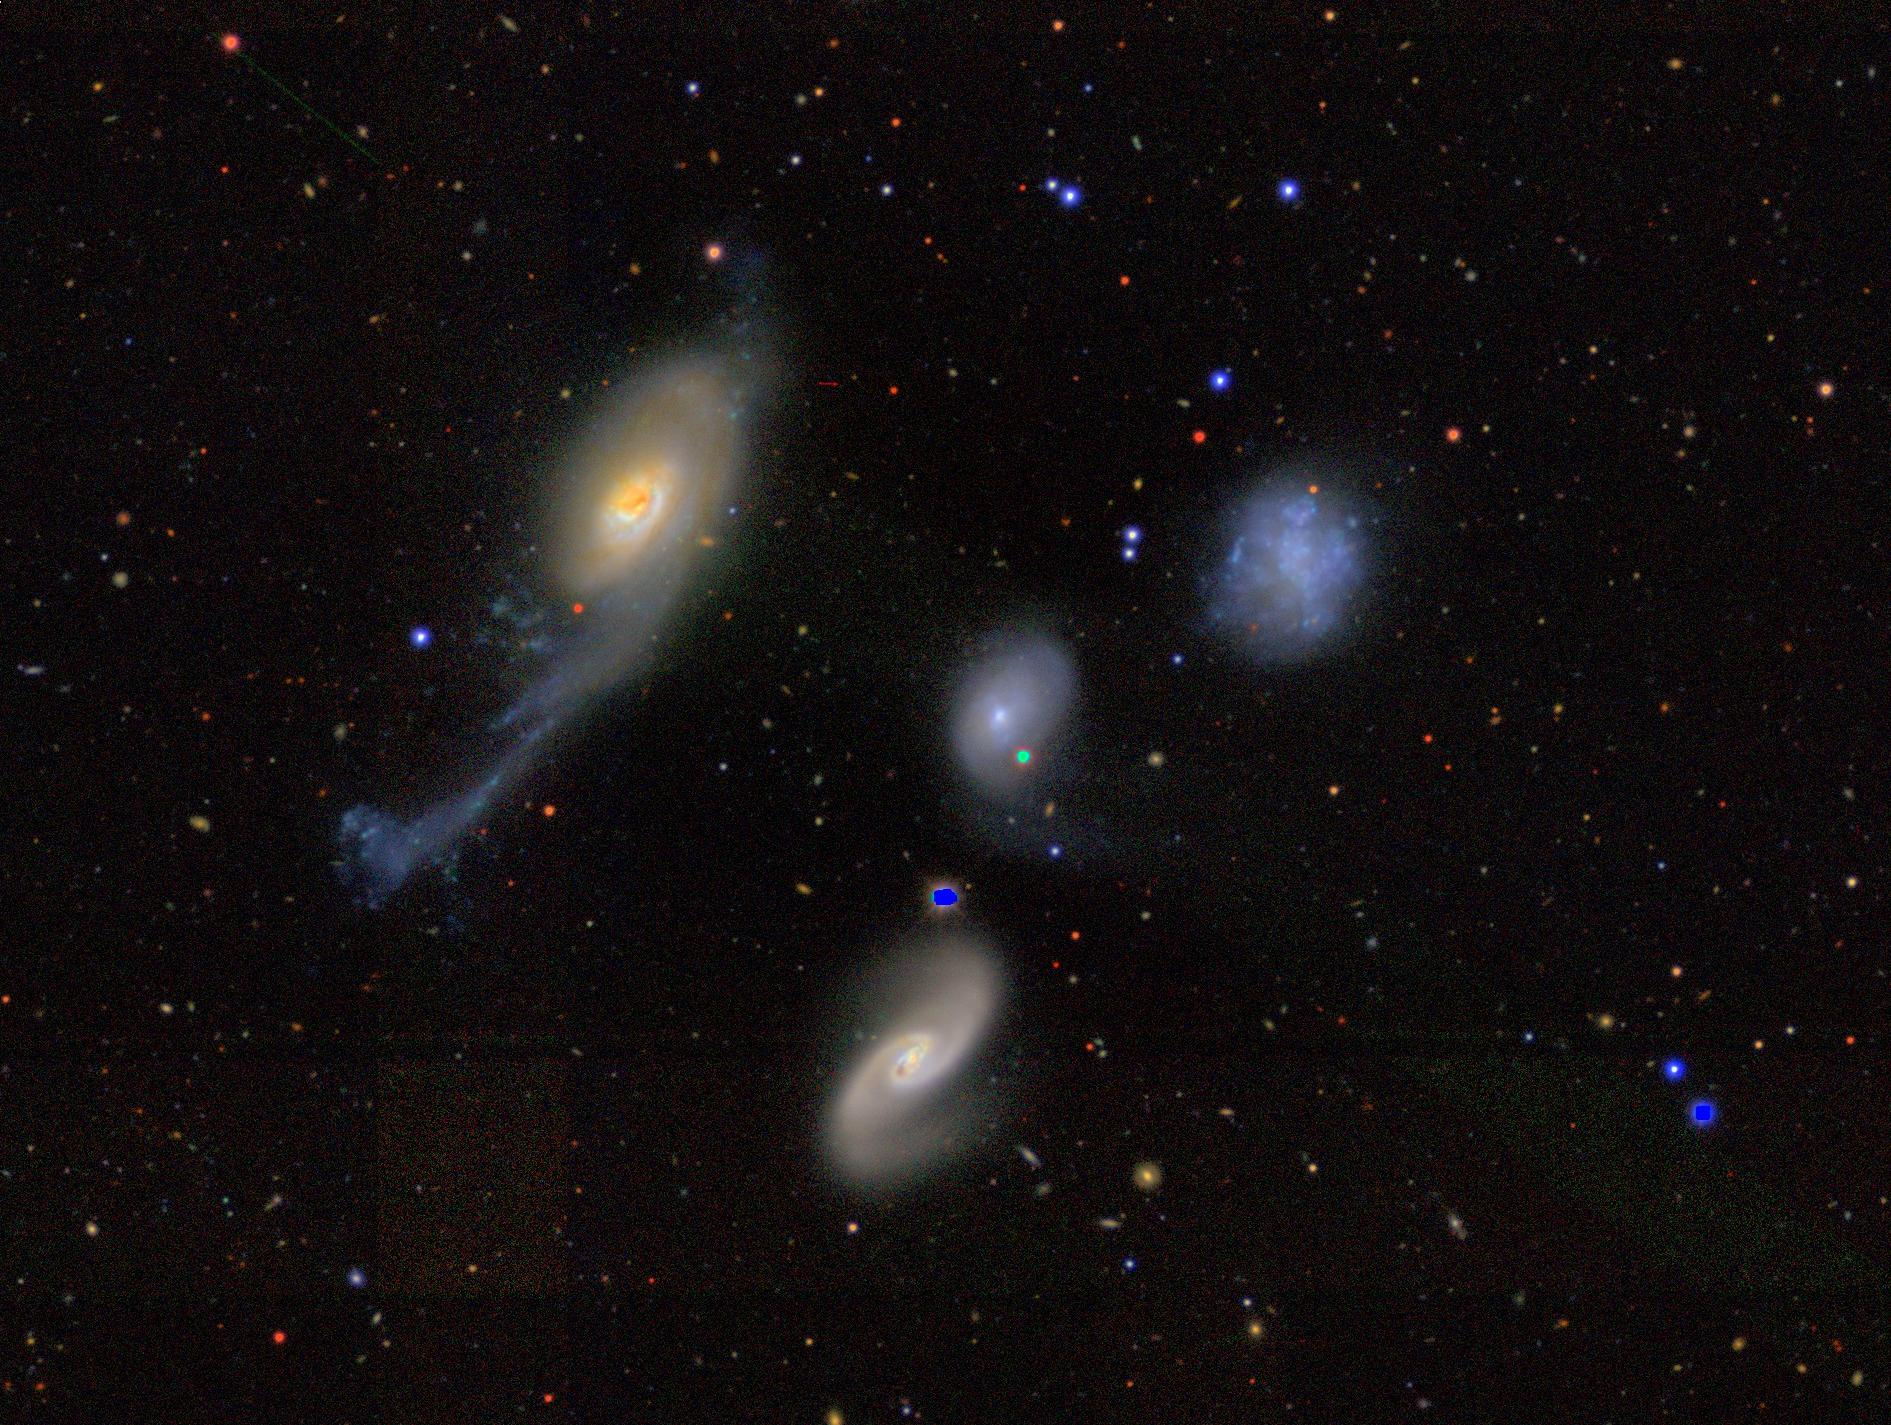
\includegraphics[width=\linewidth]{DES0022-4831-four.jpg}
                \newline
                {\tiny DES/Erin Sheldon}
        \end{column}

    \end{columns}


}



{
    \usebackgroundtemplate{%
        \colorbox{black}{ \parbox[c][\paperheight][c]{\paperwidth}{\centering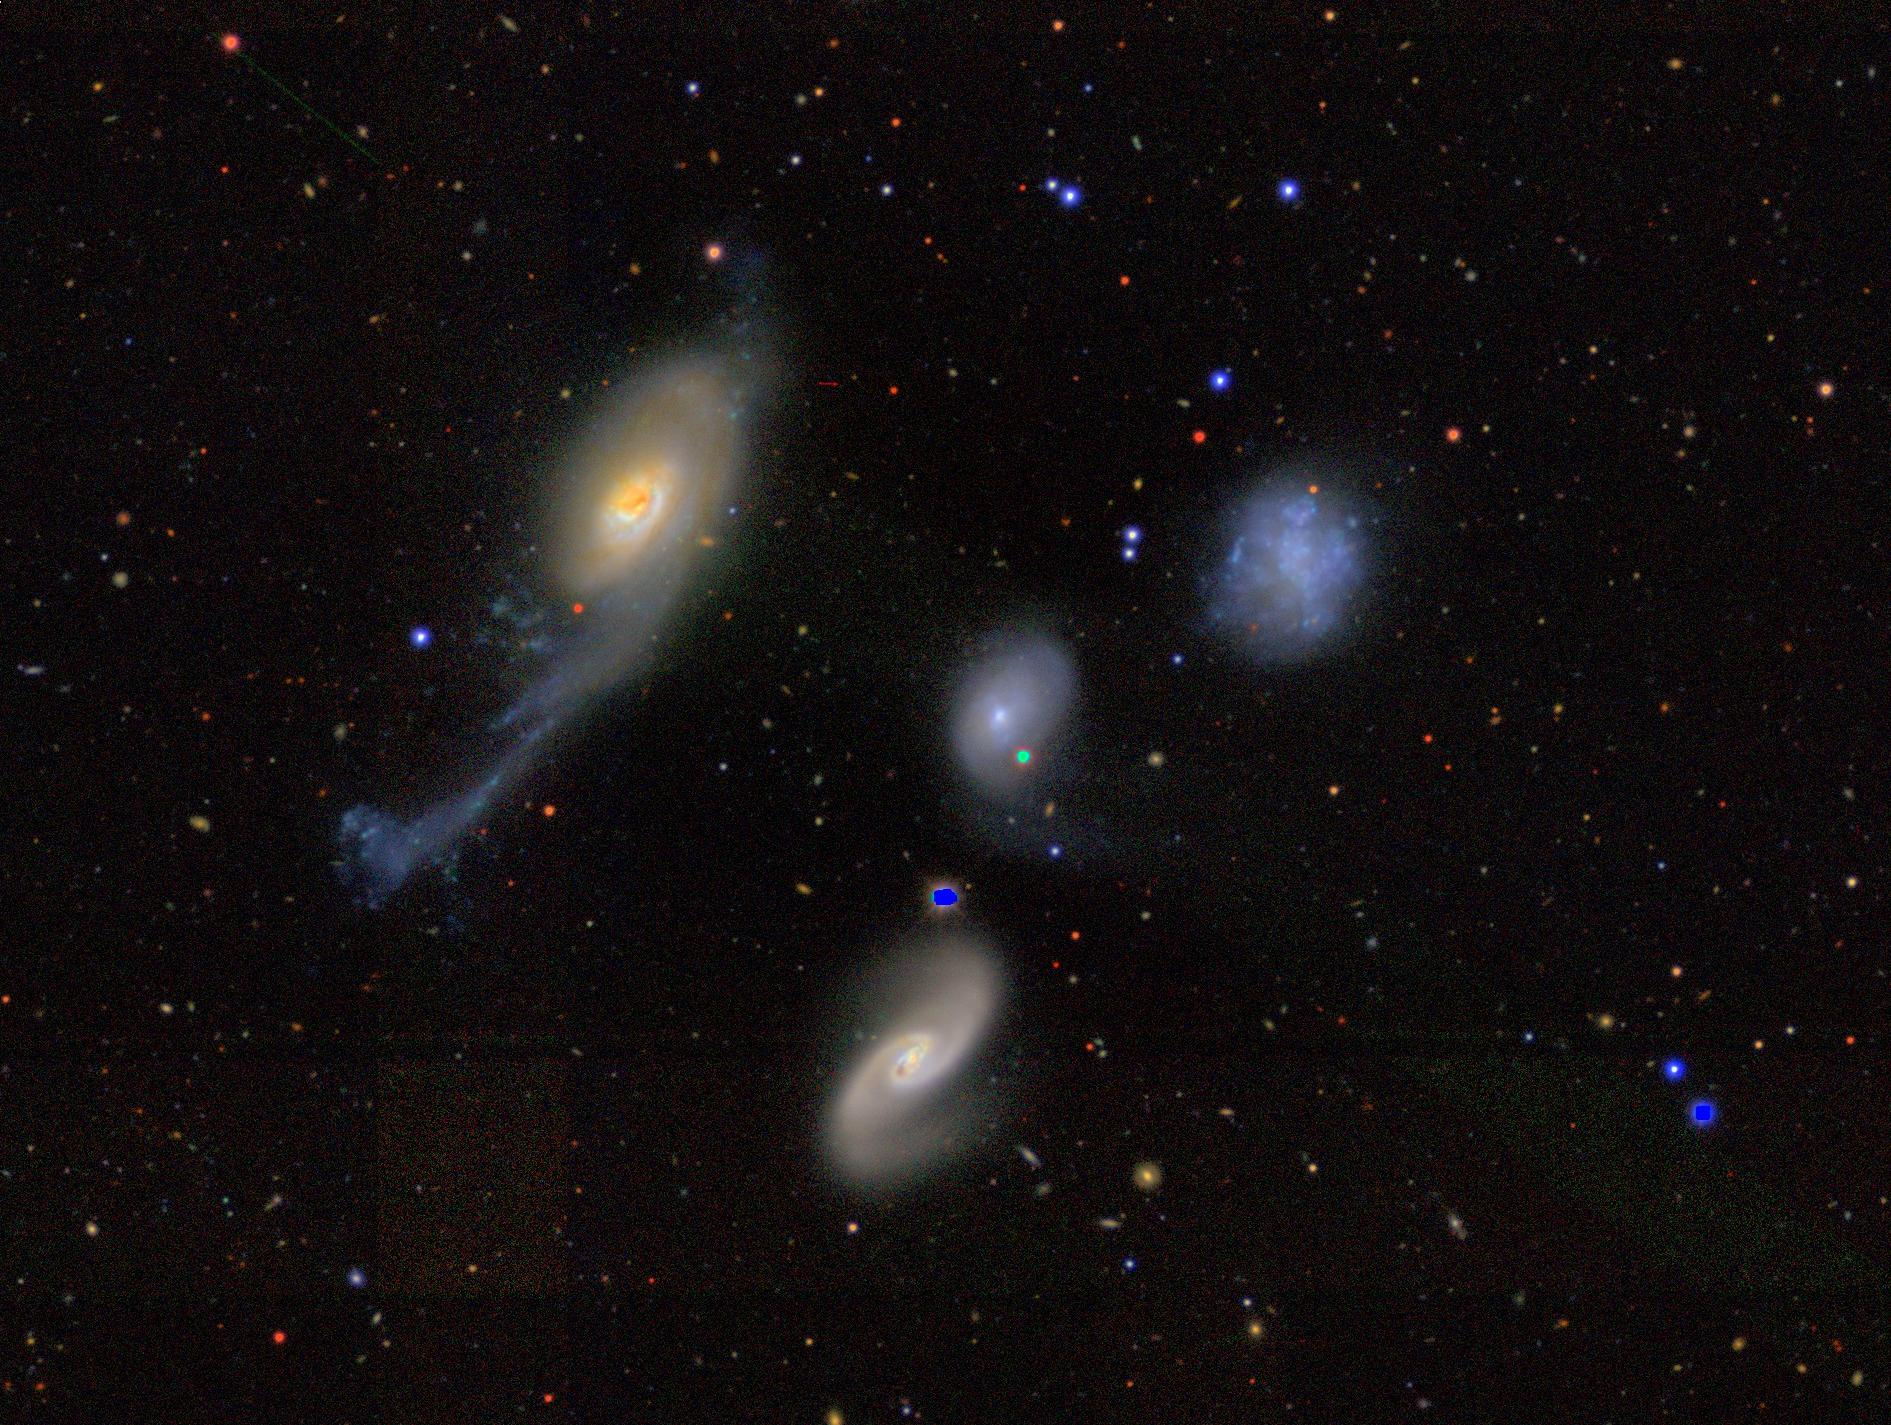
\includegraphics[height=\paperheight]{DES0022-4831-four.jpg}} }
        %\colorbox{black}{ \vbox to \paperheight{\vfil\hbox to \paperwidth{\hfil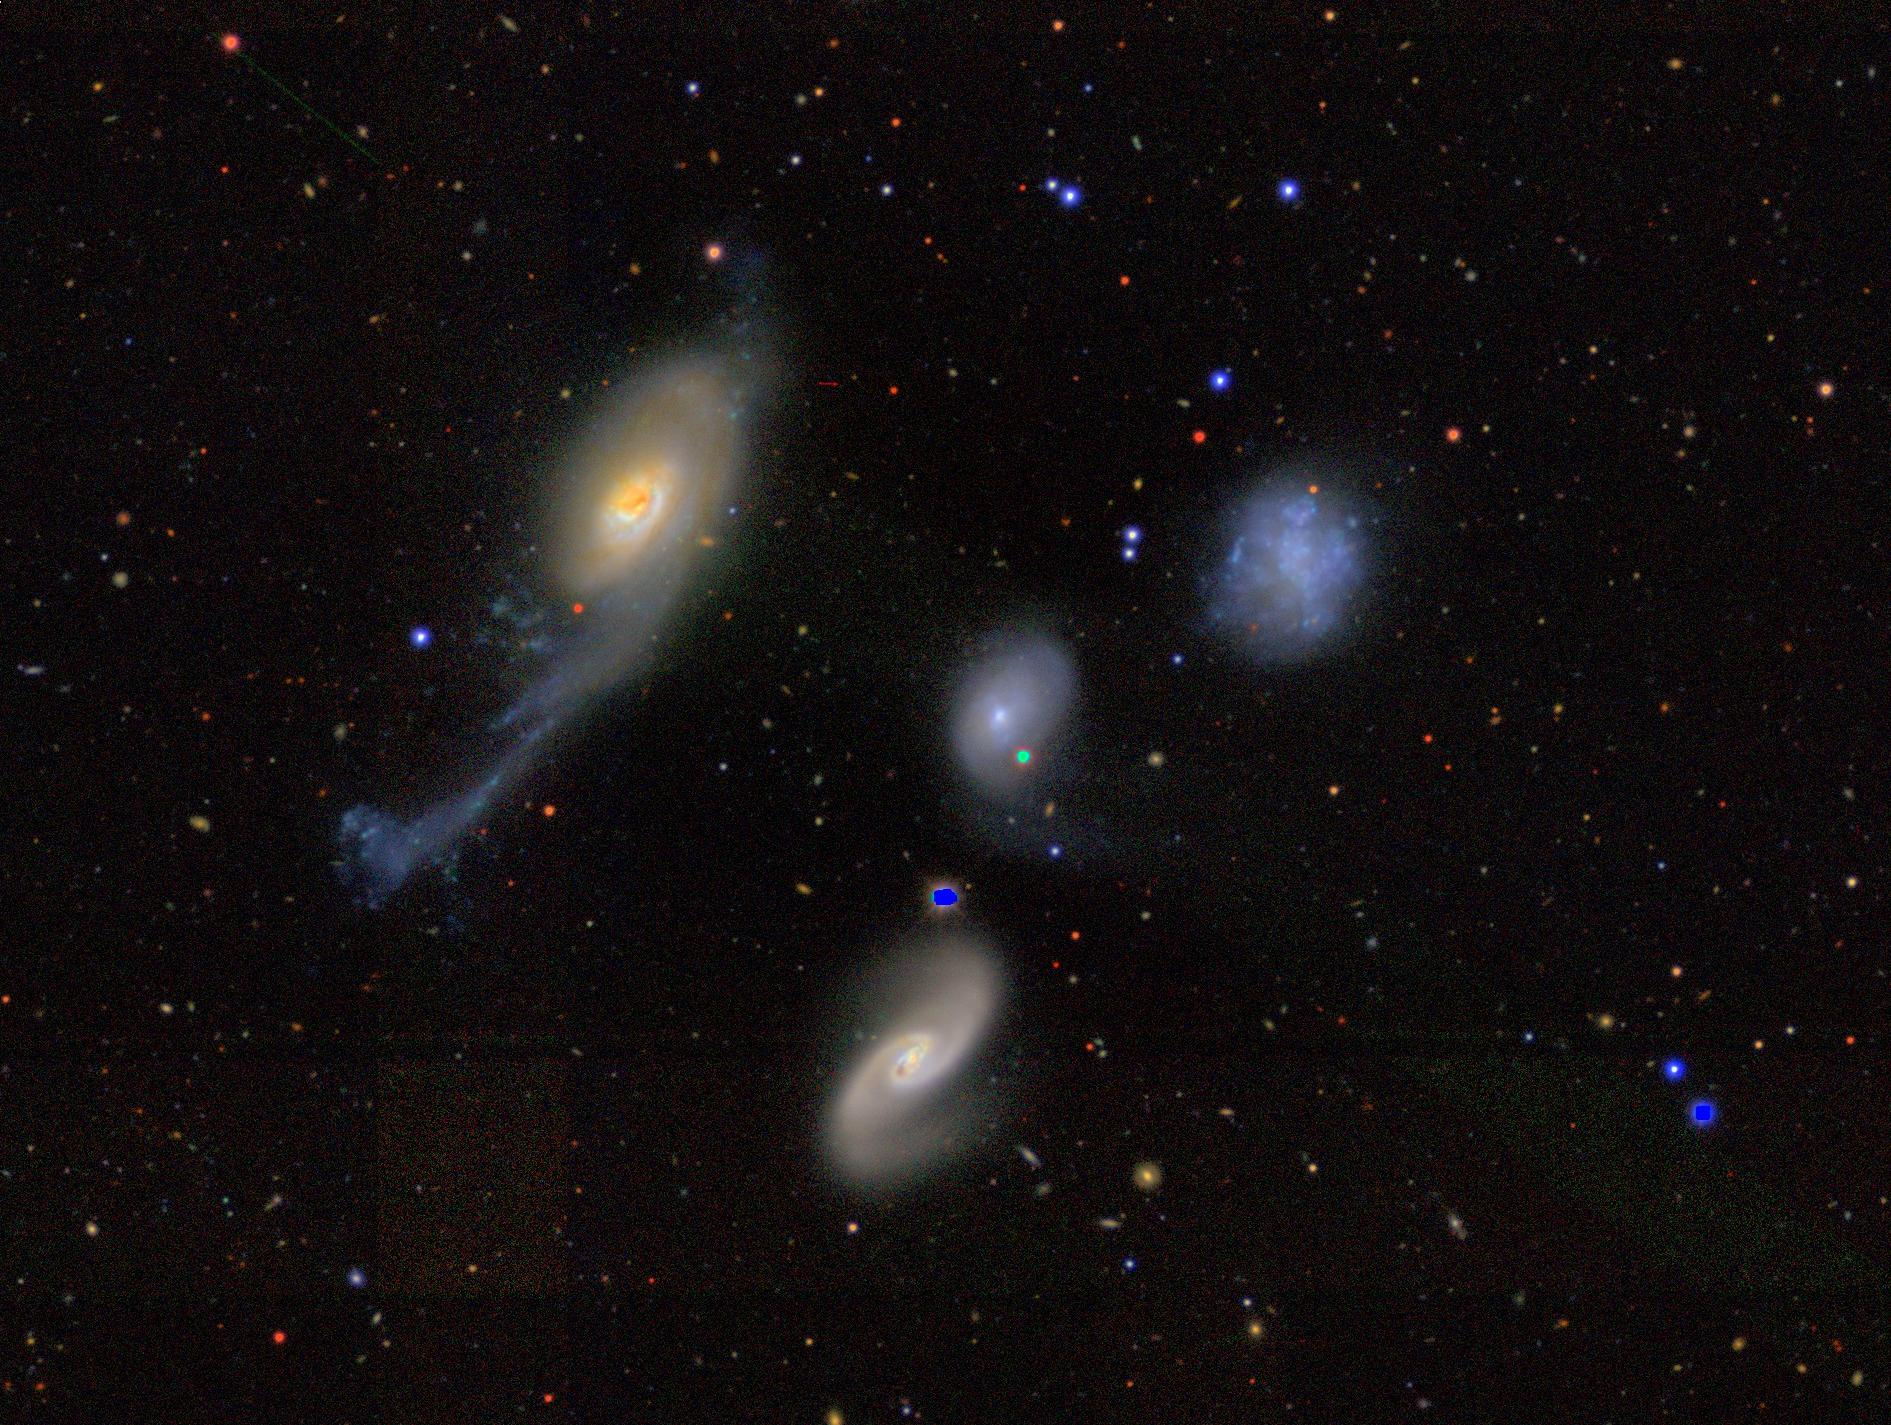
\includegraphics[height=\paperheight]{DES0022-4831-four.jpg}\hfil}\vfil} }
    }
\frame
{
}
}


{
    \usebackgroundtemplate{%
        \includegraphics[height=\paperheight]{DES-2013-01-medres.jpg}}
\frame
{
}
}

{
    \usebackgroundtemplate{%
        \colorbox{black}{ \parbox[c][\paperheight][c]{\paperwidth}{\centering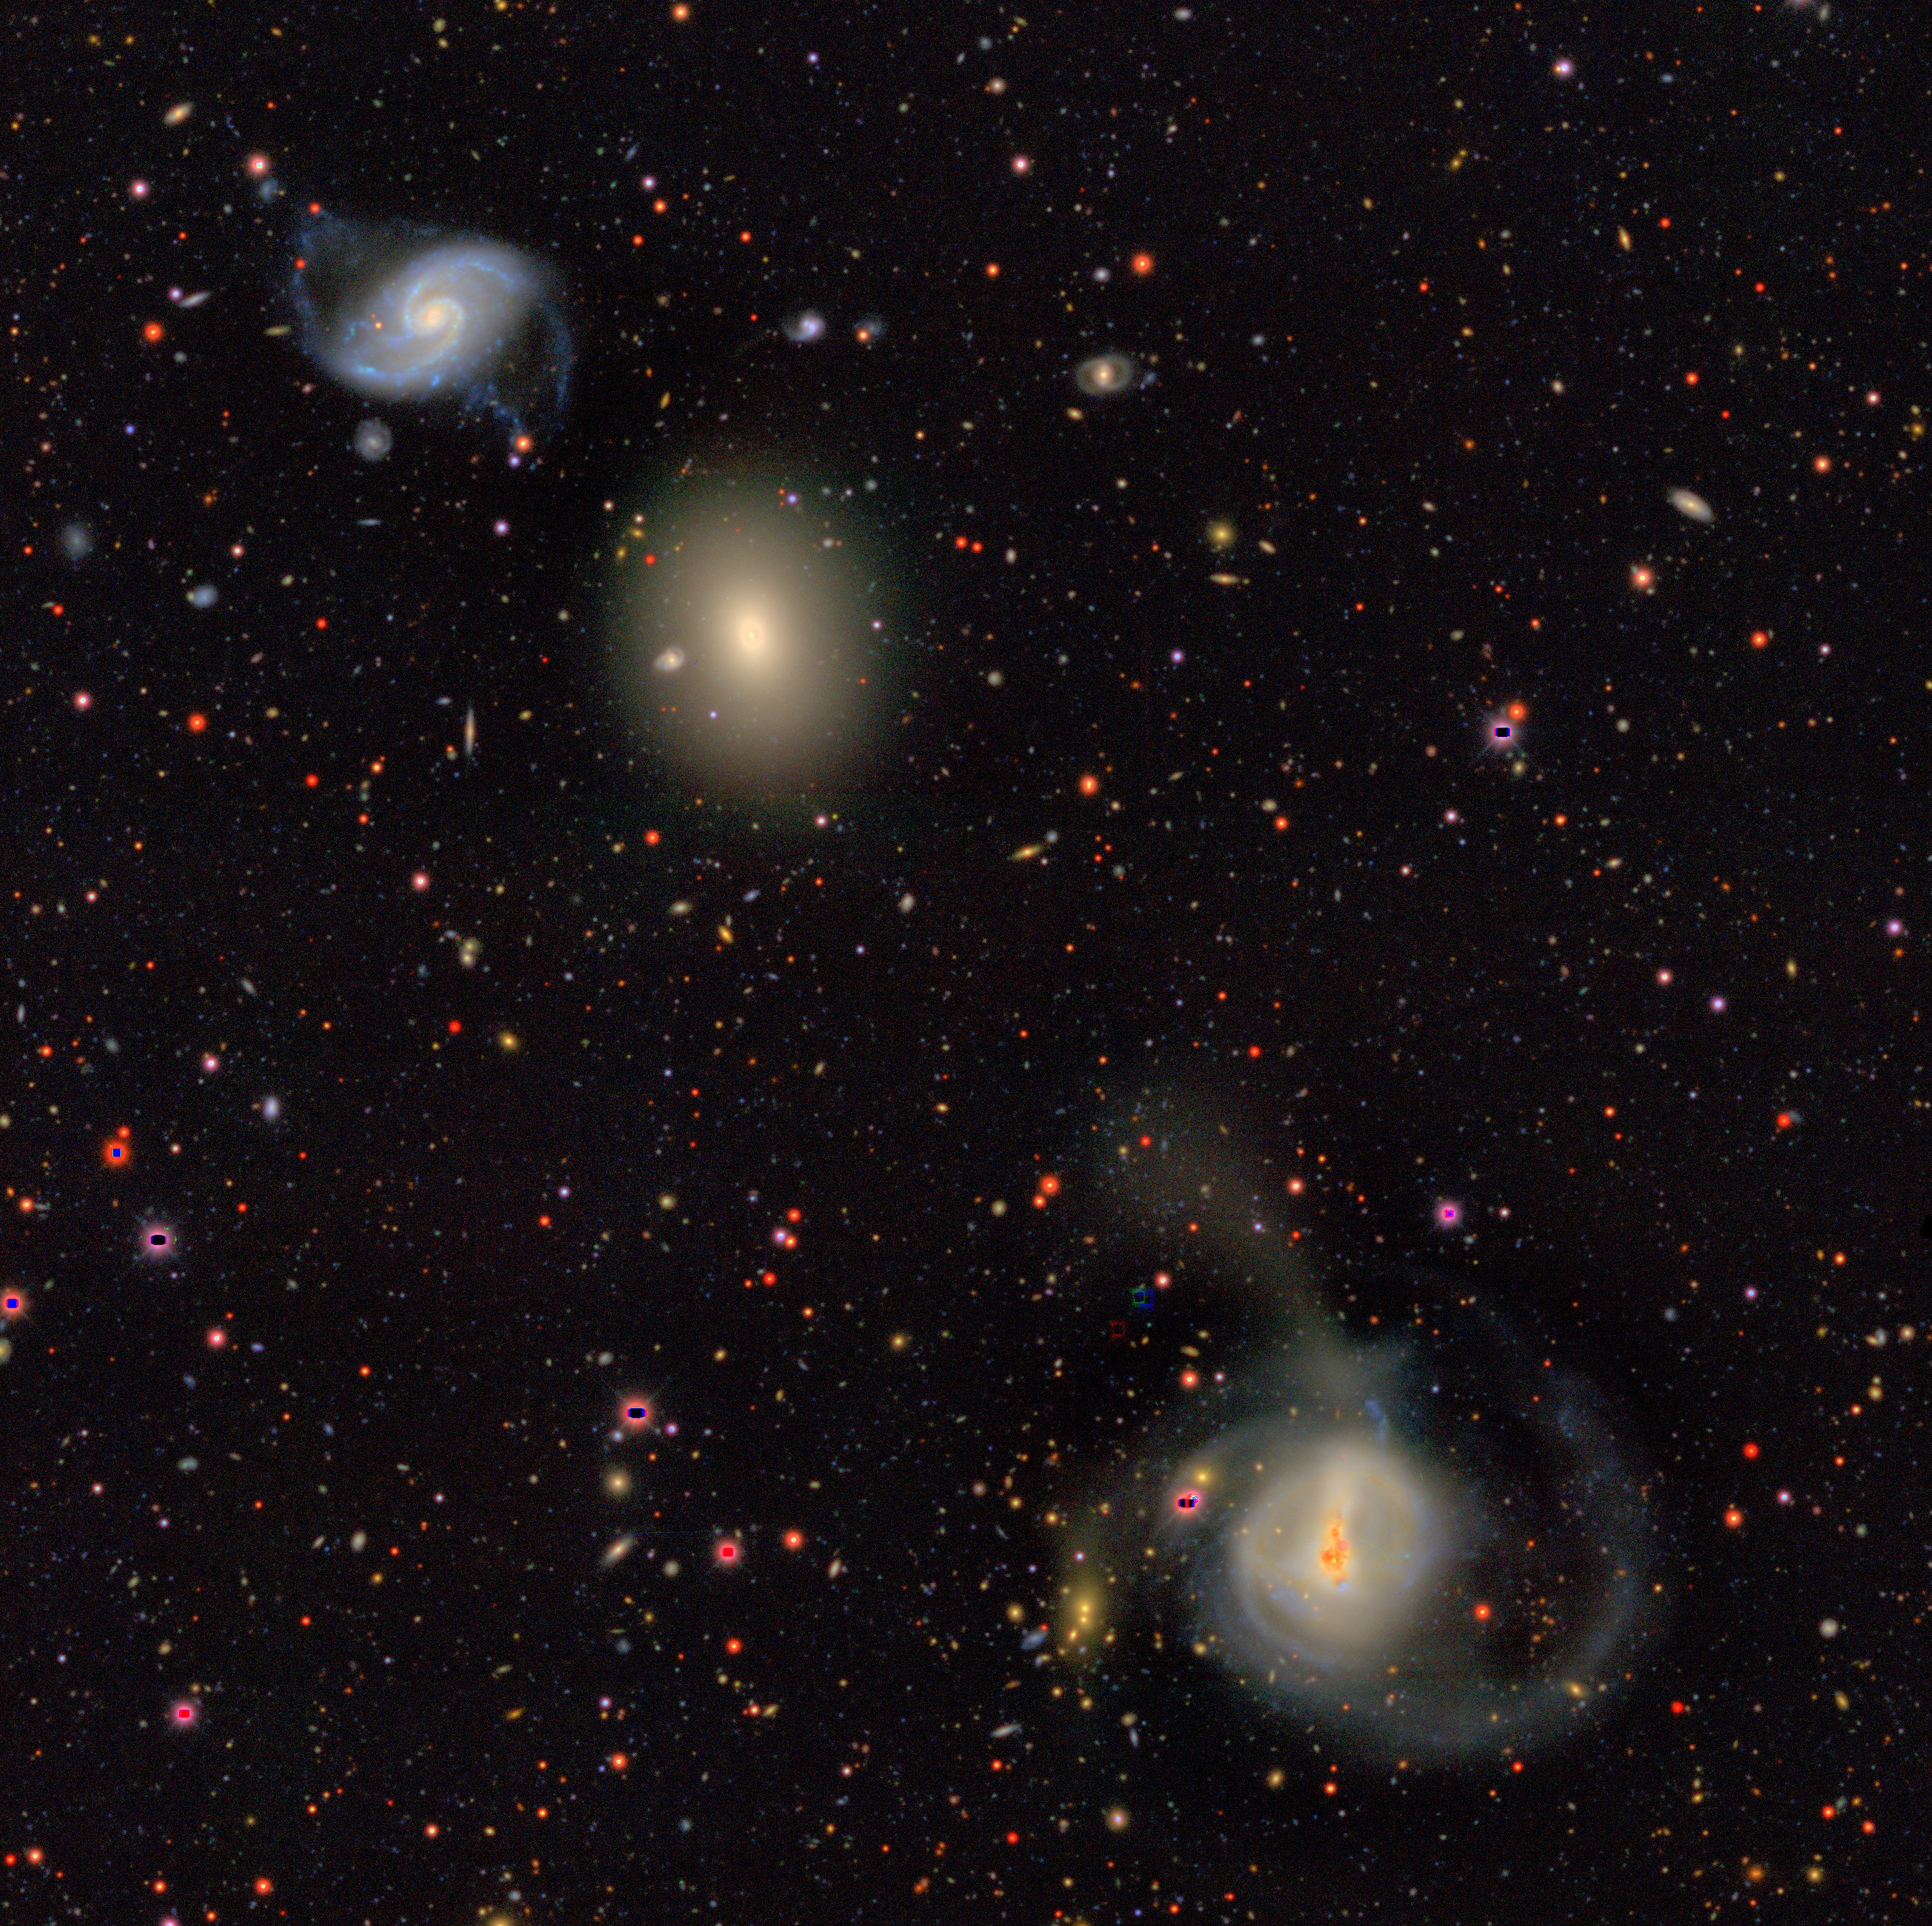
\includegraphics[height=\paperheight]{DES0428-4748_gri_sv_mask_streaks_color_trim.jpg}} }
    }
\frame
{
}
}

{
    \usebackgroundtemplate{%
        \colorbox{black}{ \parbox[c][\paperheight][c]{\paperwidth}{\centering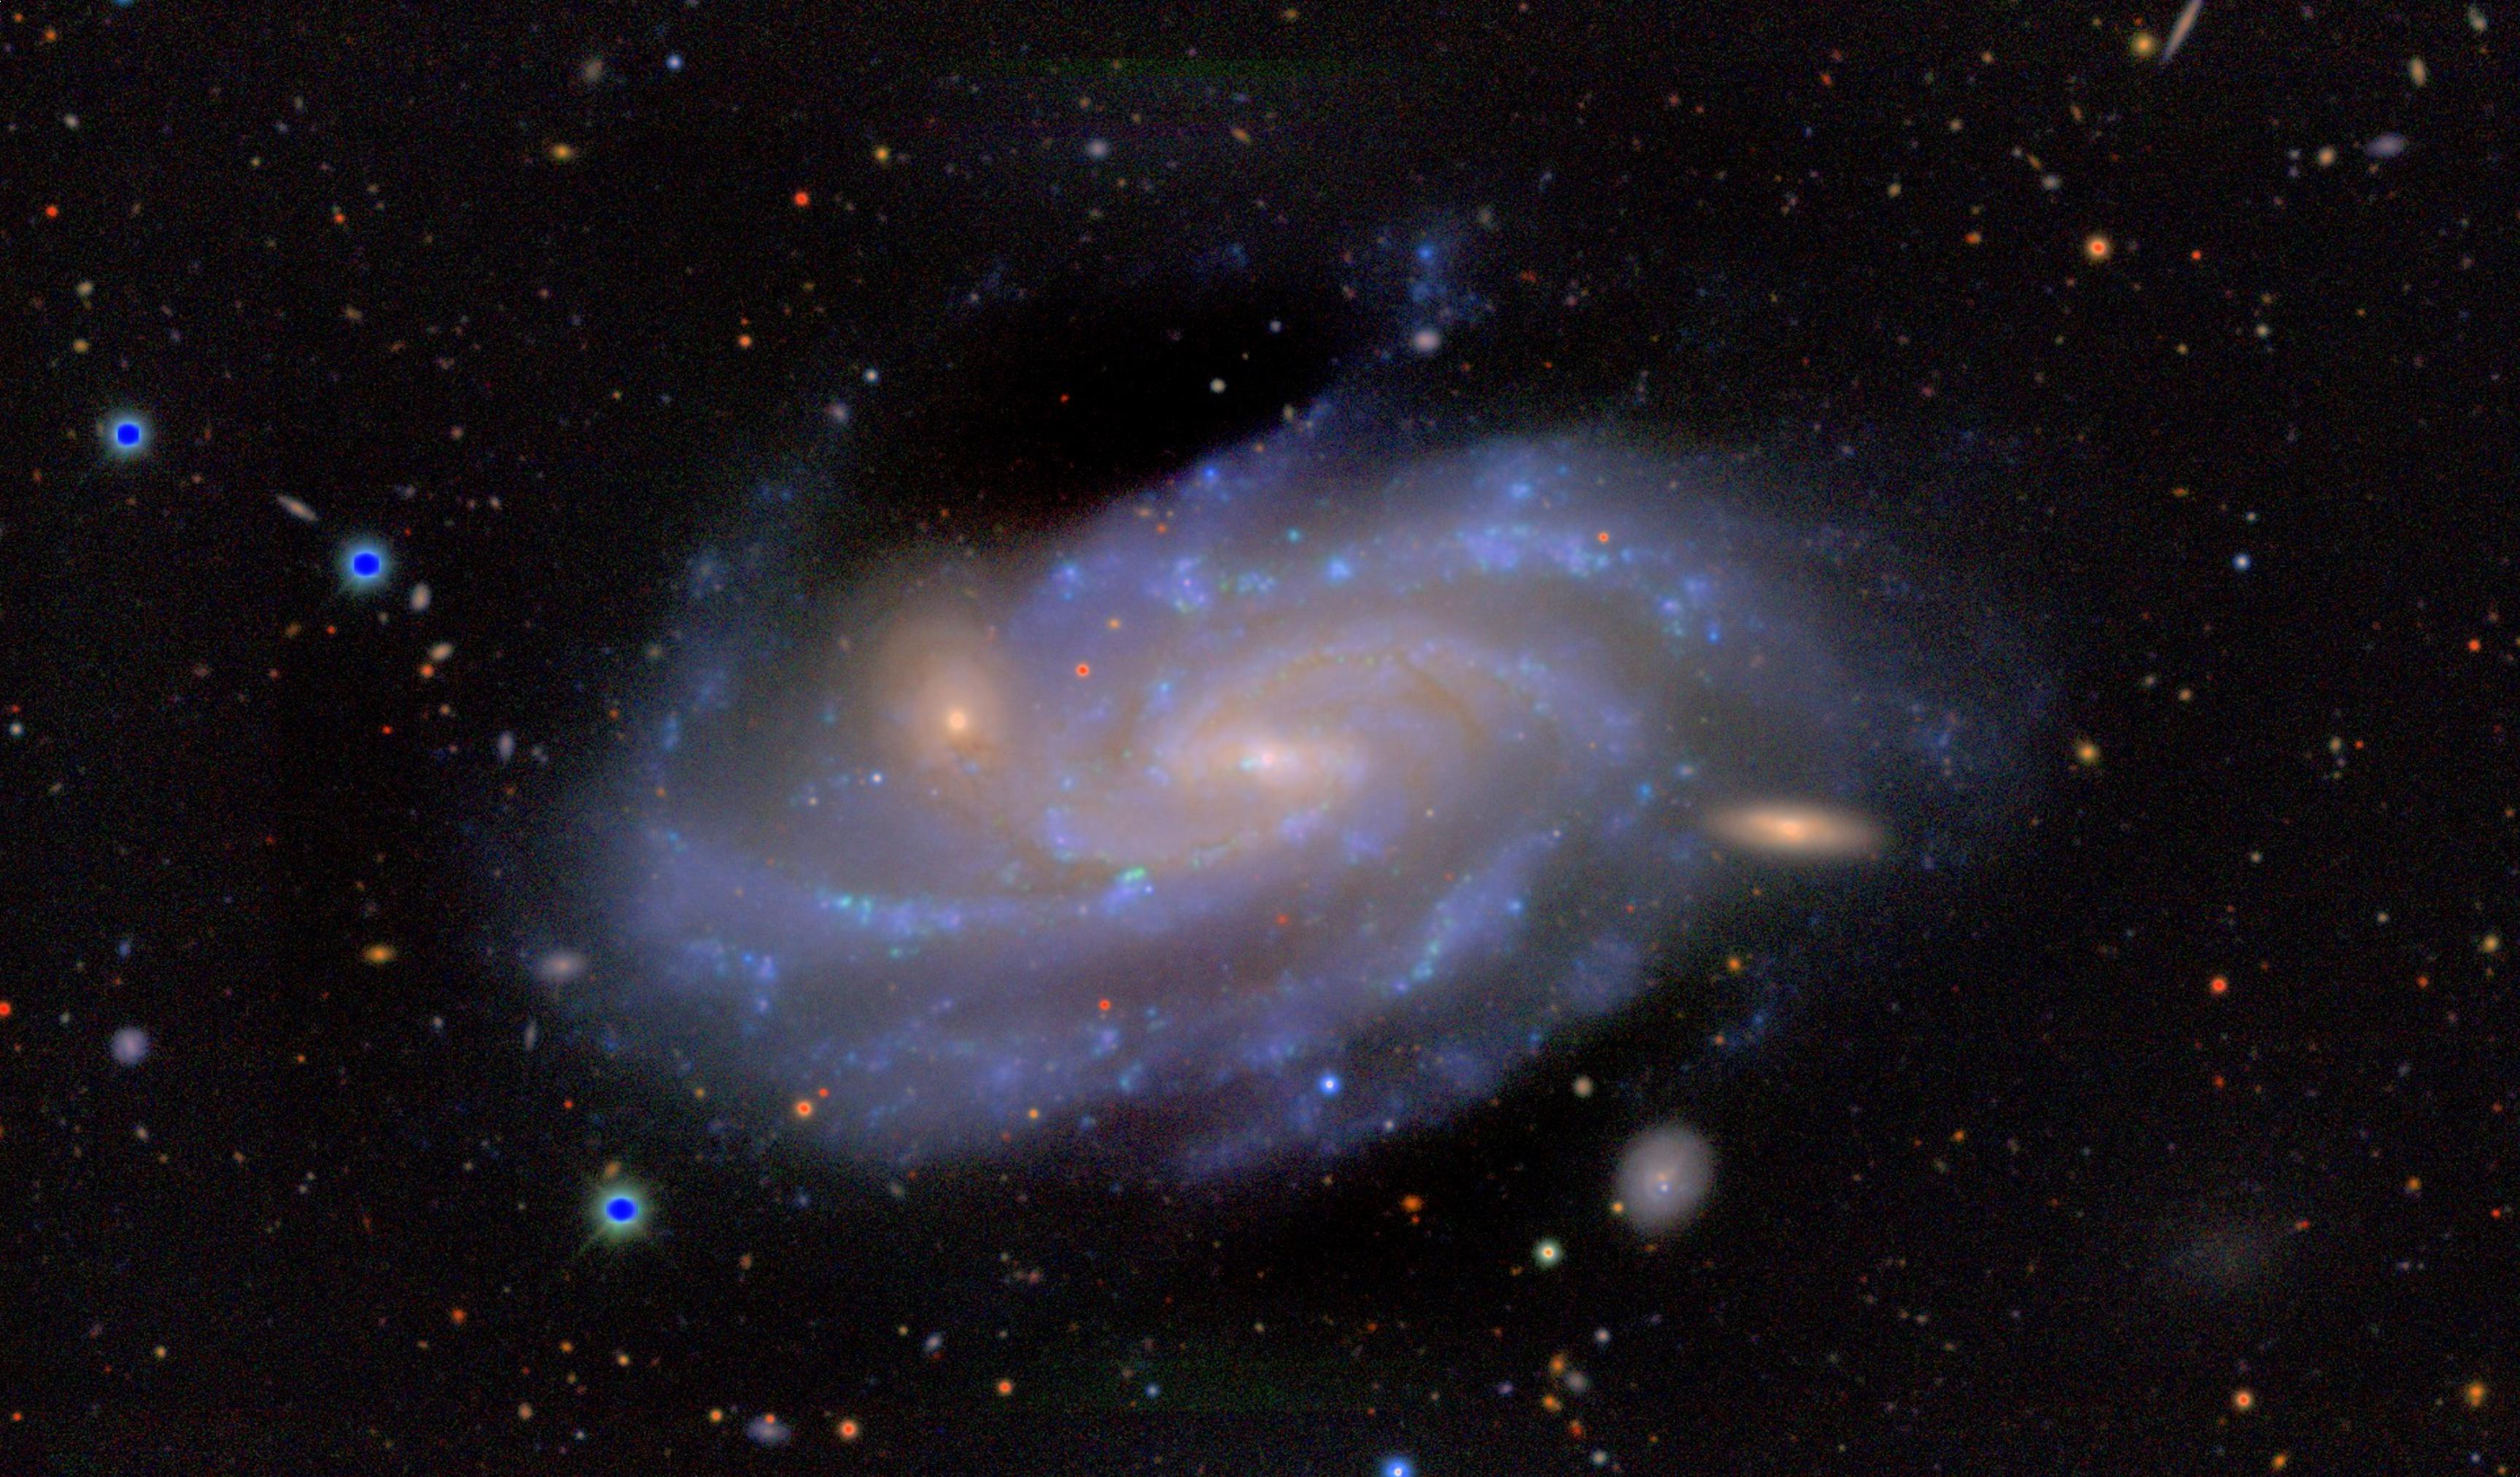
\includegraphics[height=\paperheight]{DES0130-2249-nearby-projection.jpg}} }
    }
\frame
{
}
}

{
    \usebackgroundtemplate{%
        \colorbox{black}{ \parbox[c][\paperheight][c]{\paperwidth}{\centering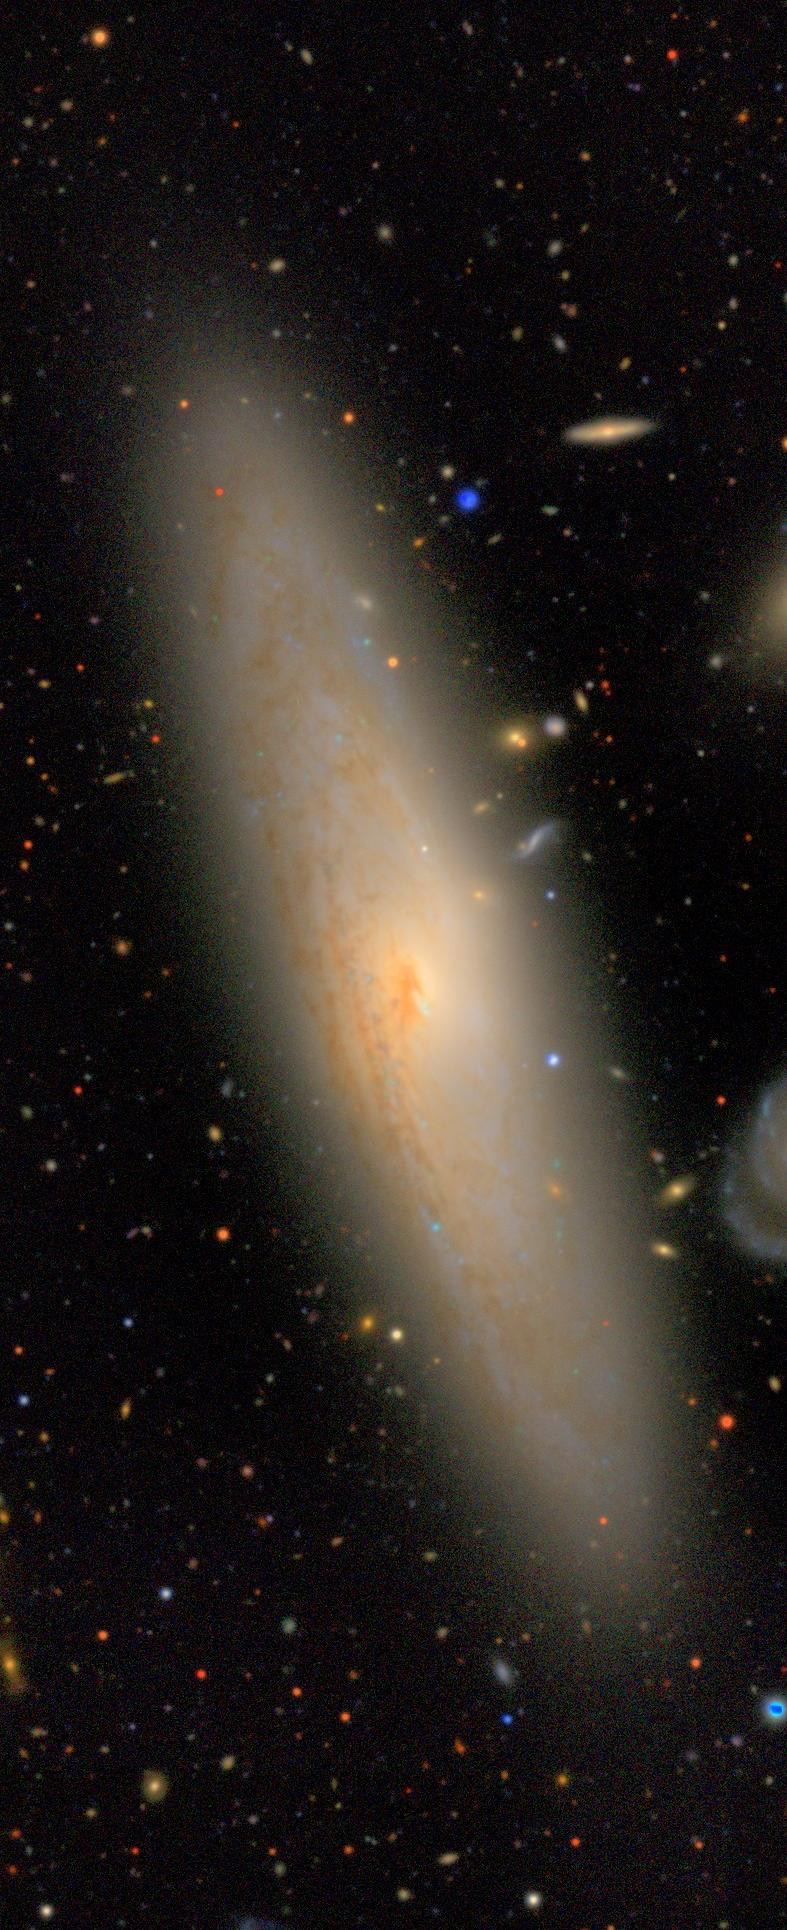
\includegraphics[width=0.7\paperheight,angle=90]{DES0406-5414-huge.jpg}} }
    }
\frame
{
}
}

{
    \usebackgroundtemplate{%
        \colorbox{black}{ \parbox[c][\paperheight][c]{\paperwidth}{\centering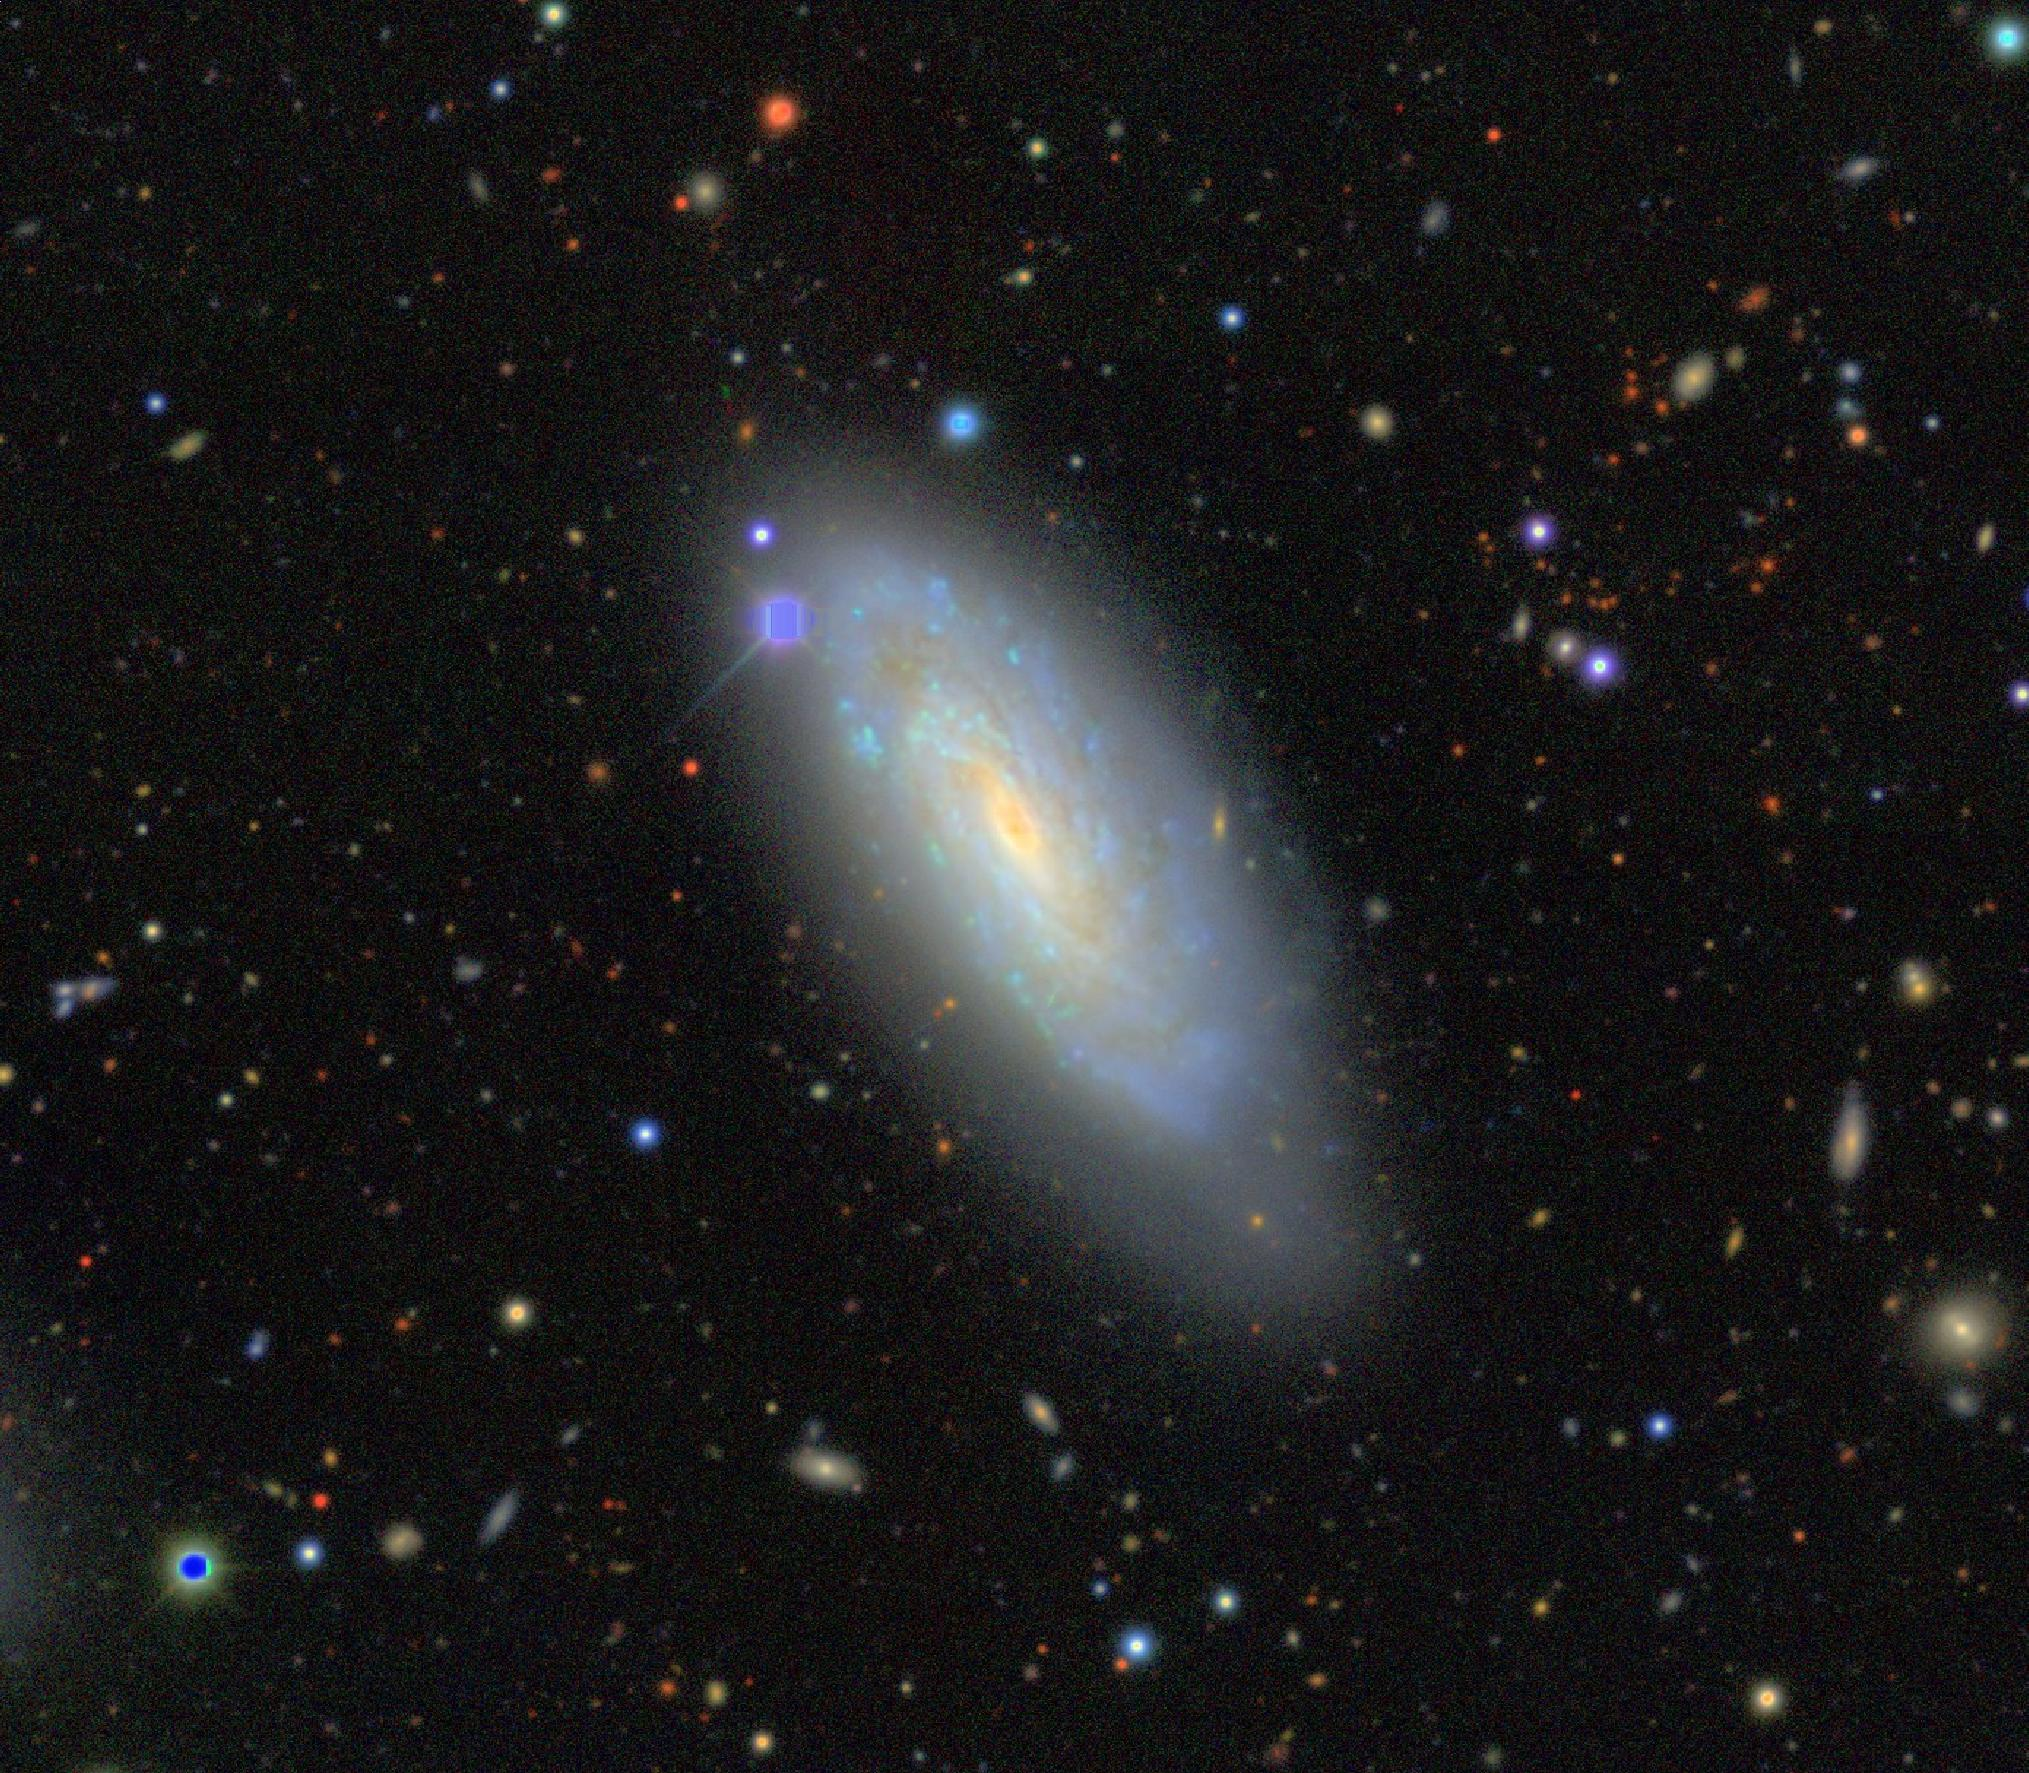
\includegraphics[height=\paperheight]{DES2320-4206-spiral.jpg}} }
    }
\frame
{
}
}


\frame
{

    \frametitle{DES Year 1 Cosmology Results}

    %\setbeamerfont*{itemize/enumerate body}{size=\large}

    \begin{columns}
        \begin{column}{0.5\textwidth}
            \begin{itemize}

                \item Year 1 Cosmology results using lensing and galaxy clustering are out
                    \begin{itemize}
                        \item Cosmic shear (shear correlation function)
                        \item Galaxy density correlation function
                        \item Galaxy-shear cross correlation function
                    \end{itemize}

                \item Shear and photometry measurements by Erin Sheldon of BNL

            \end{itemize}

        \end{column}
        \begin{column}{0.5\textwidth}
            \centering
                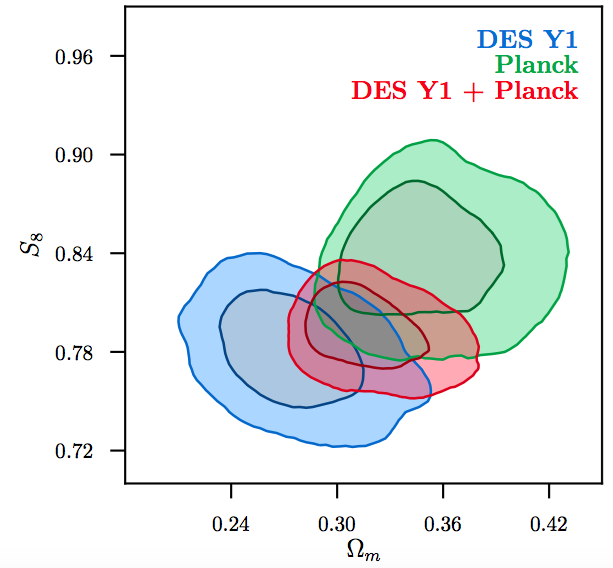
\includegraphics[width=\linewidth]{3x2-fig10.png}
                \newline
                {\tiny DES Collaboration 2018}
        \end{column}

    \end{columns}

}

\frame
{

    \frametitle{DES Shear Catalog: \Mcal}

    %\setbeamerfont*{itemize/enumerate body}{size=\large}

    \begin{columns}
        \begin{column}{0.5\textwidth}
            \begin{itemize}

                \item New shear measurement technique \mcal\ (Sheldon \& Huff
                    2017)

                \item First method demonstrated to be accurate enough for
                    current and future lensing surveys (LSST).

                \item Implemented in DES by Erin Sheldon.  Code 
                    is free software available as part of the \ngmix\ package.

                \item All measurements done by Sheldon using mainly BNL contributed
                    resources (about 10\% using SLAC)

            \end{itemize}

        \end{column}
        \begin{column}{0.5\textwidth}
            \centering
                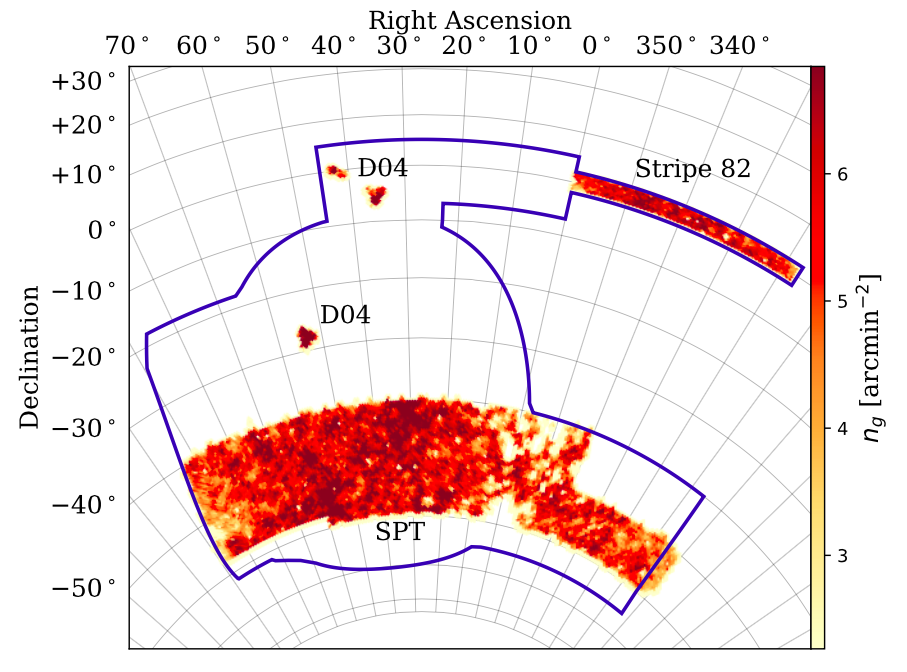
\includegraphics[width=\linewidth]{shearcat-fig2.png}
                \newline
                {\tiny Zunts, Sheldon et al. 2018}
        \end{column}

    \end{columns}

}

\frame
{

    \frametitle{DES Photometry}

    %\setbeamerfont*{itemize/enumerate body}{size=\large}

    \begin{columns}
        \begin{column}{0.5\textwidth}
            \begin{itemize}

                \item Multi-object fitting:  New object deblender developed by
                    Sheldon and Matt Becker using \ngmix

                \item Assigns the light appropriately to each member of a group
                    of objects.

                \item Used as primary photometry in DES
                    \begin{itemize}

                        \item Used for as flux measurements for photometric
                            redshift determination

                        \item Used to define the galaxies in
                            the large scale structure sample

                        \item Used in the RedMapper galaxy cluster
                            finder.

                    \end{itemize}

                \item Deblended images are a crucial input for \mcal.

            \end{itemize}

        \end{column}
        \begin{column}{0.5\textwidth}
            \centering
                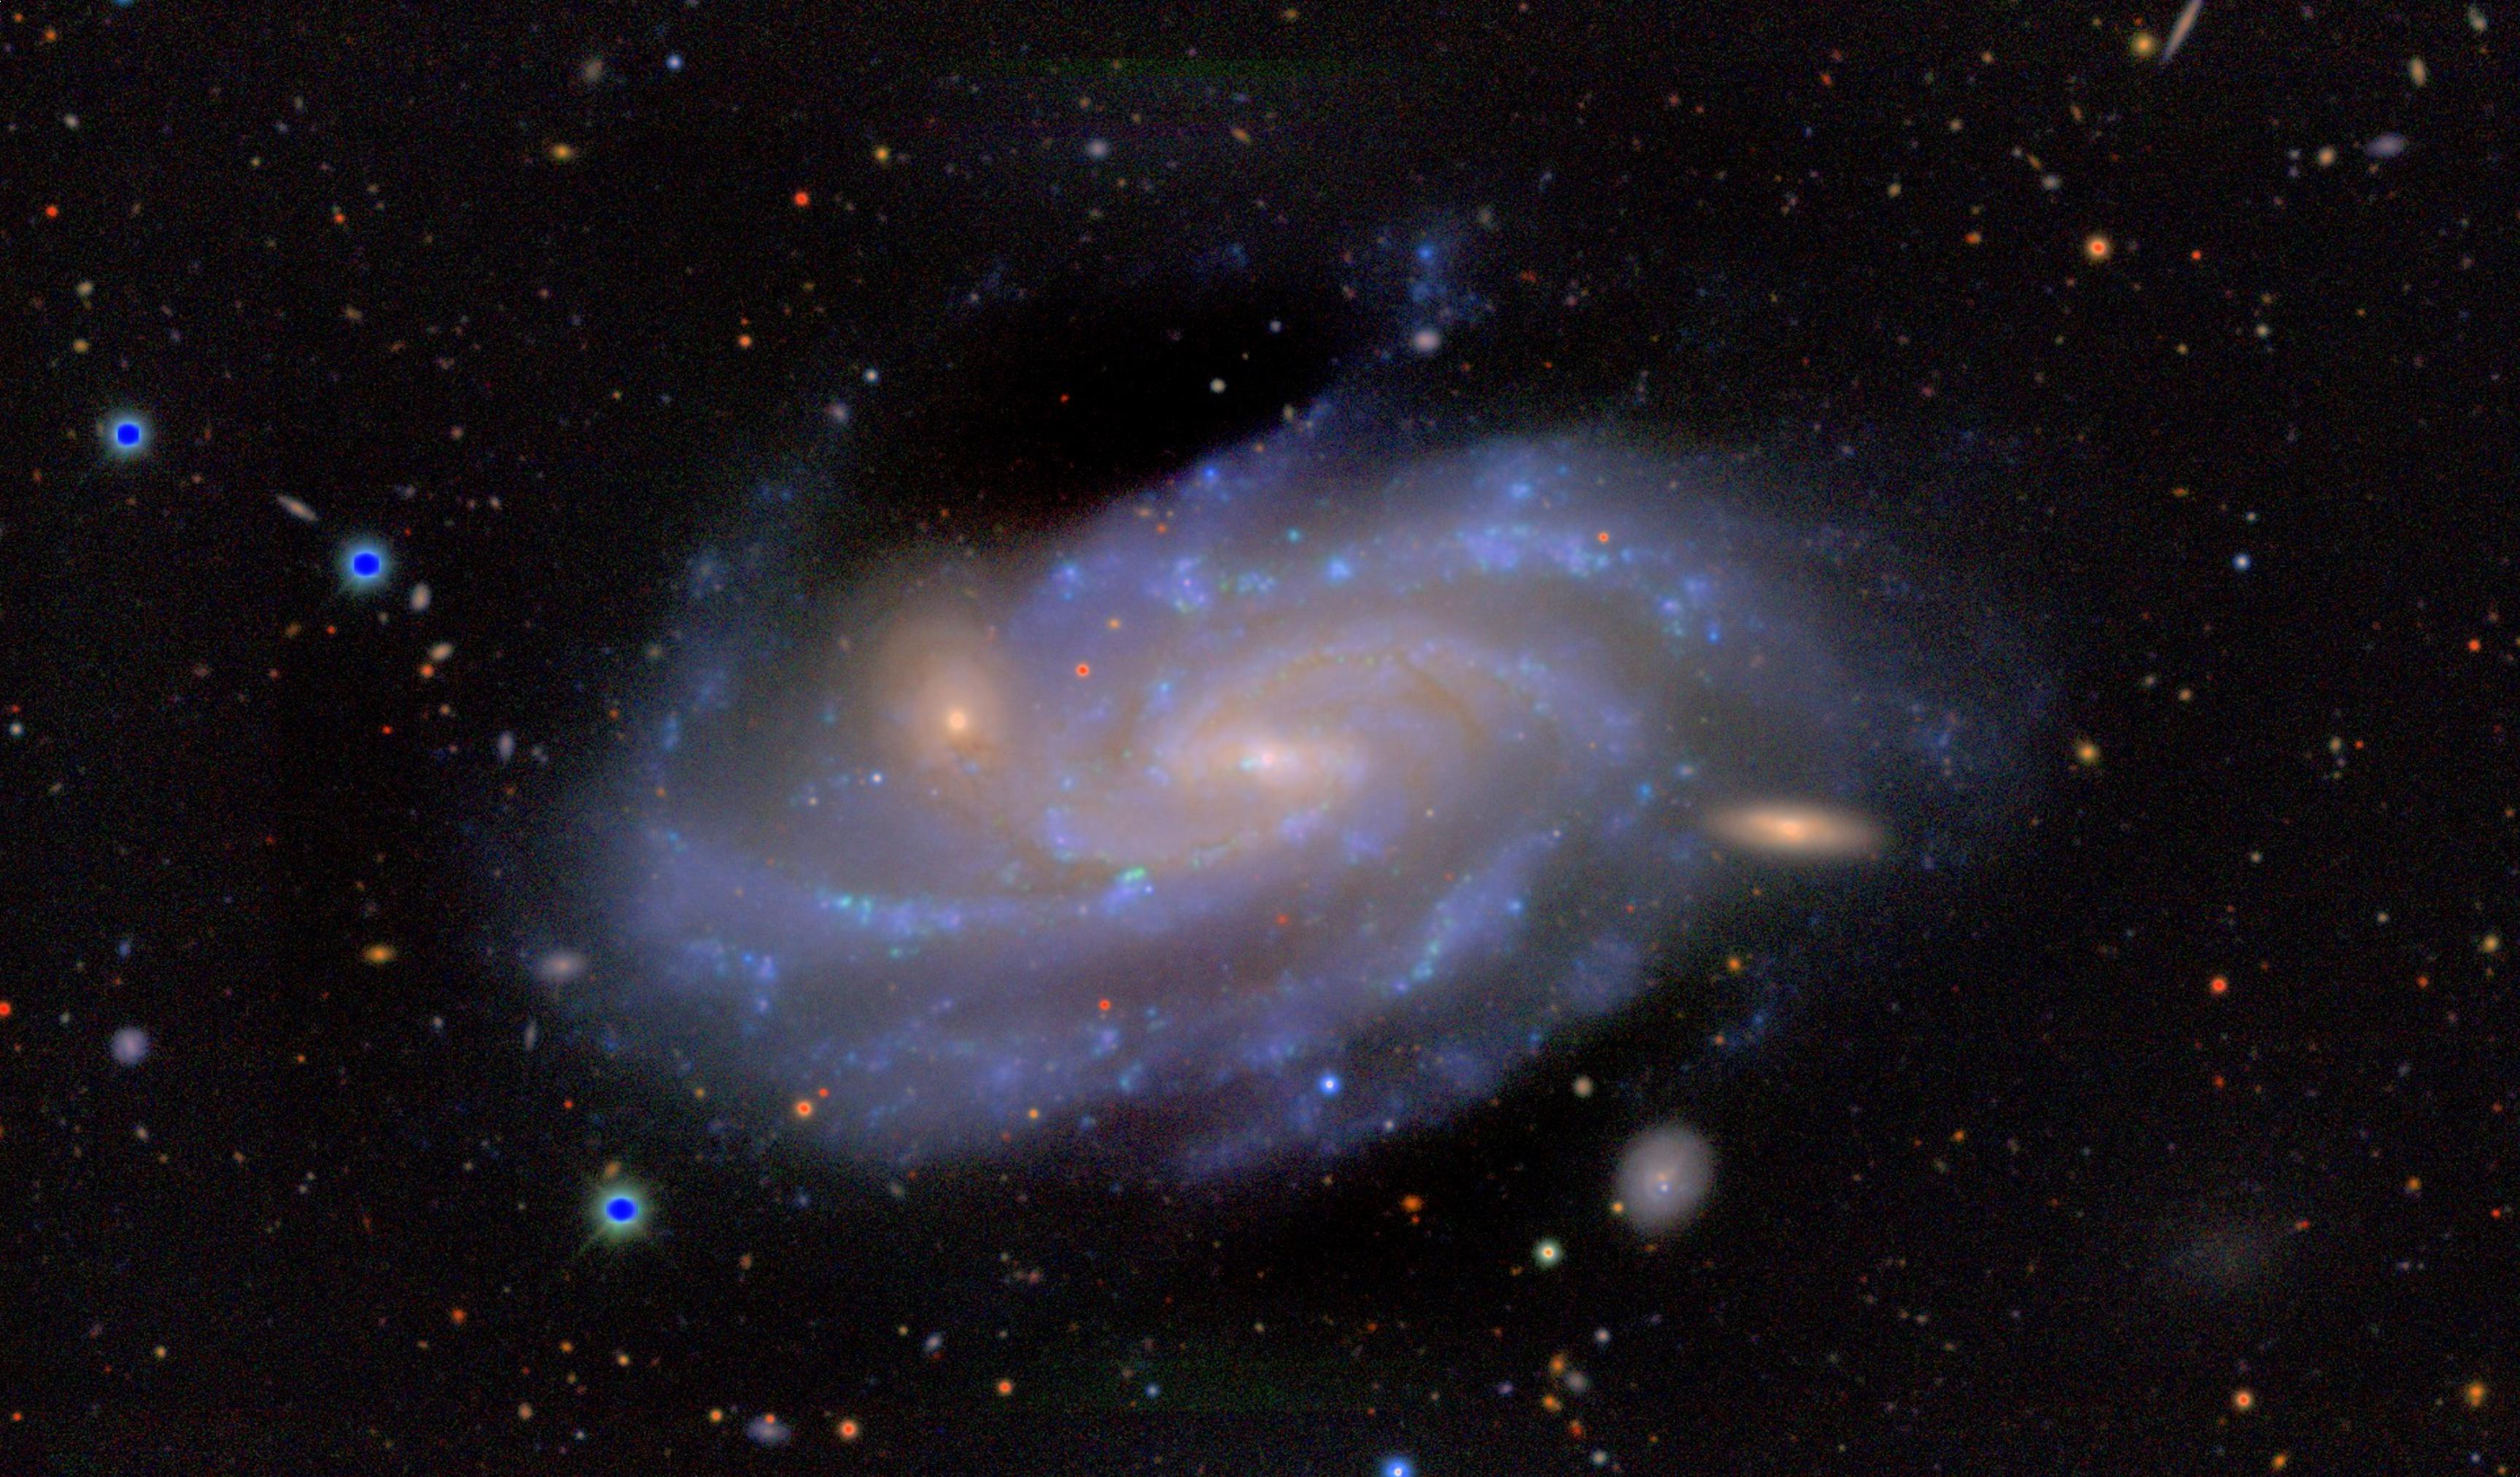
\includegraphics[width=\linewidth]{DES0130-2249-nearby-projection.jpg}
                \newline
                {\tiny Hoyle et al. 2018}
        \end{column}

    \end{columns}

}

\frame
{

    \frametitle{Cosmic Shear}

    %\setbeamerfont*{itemize/enumerate body}{size=\large}

    \begin{columns}
        \begin{column}{0.5\textwidth}
            \begin{itemize}

                \item Cosmic shear is basically the correlation
                    function of the shear.

                \item This is the most powerful probe used in the
                    recent DES Year1 Cosmology results

                \item The primary shear catalog was \mcal.  We also
                    had a comparision code \imshape\ which we
                    found to give consistent results.

                \item Most accurate and precise cosmic shear measurements to
                    date.

            \end{itemize}

        \end{column}
        \begin{column}{0.5\textwidth}
            \centering
                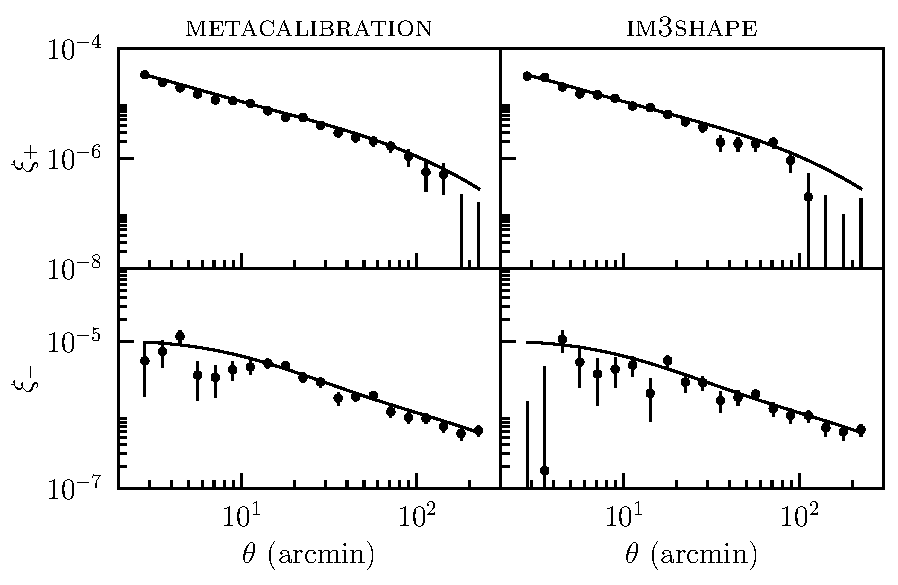
\includegraphics[width=\linewidth]{xi_notomo.pdf}
                \newline
                {\tiny Troxel et al. 2018}
        \end{column}

    \end{columns}

}

\frame
{

    \frametitle{Galaxy-shear Cross Correlations}

    %\setbeamerfont*{itemize/enumerate body}{size=\large}

    \begin{columns}
        \begin{column}{0.5\textwidth}
            \begin{itemize}

                \item Cross-correlation between the positions
                    of luminous red galaxies and the shear.

                \item Again, the primary shear catalog was \mcal.

                \item Most accurate and precise galaxy-shear cross
                    correlations to date.

            \end{itemize}

        \end{column}
        \begin{column}{0.5\textwidth}
            \centering
                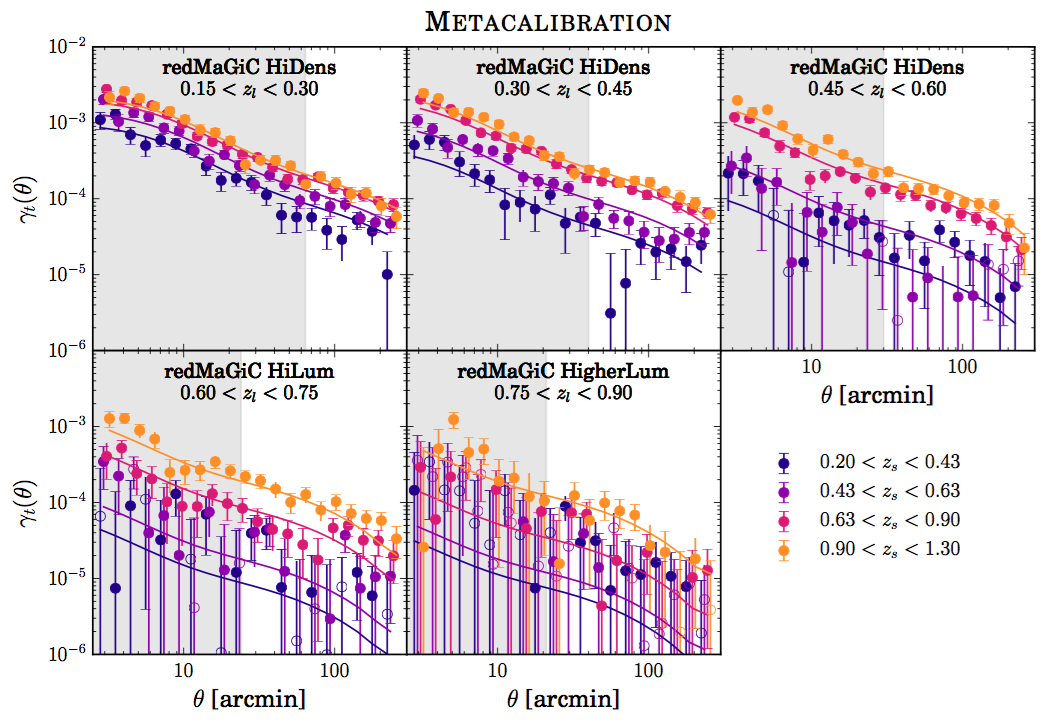
\includegraphics[width=\linewidth]{ggl-fig2a.png}
                \newline
                {\tiny Prat et al. 2018}
        \end{column}

    \end{columns}

}

\frame
{

    \frametitle{Galaxy Correlations}

    %\setbeamerfont*{itemize/enumerate body}{size=\large}

    \begin{columns}
        \begin{column}{0.5\textwidth}
            \begin{itemize}

                \item Completes the triumvirate:  auto and cross correlations
                    of galaxies and shear.

                \item The fluxes came from the MOF deblender used to define
                    the sample, which is luminous red galaxies 
                    (RedMagic; Rykoff et al).

            \end{itemize}

        \end{column}
        \begin{column}{0.5\textwidth}
            \centering
                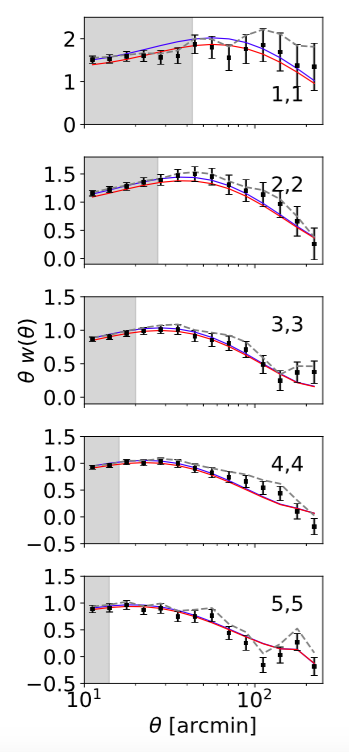
\includegraphics[height=0.9\textheight]{galclustering-fig7a.png}
                \newline
                {\tiny Elvin-Poole et al. 2018}
        \end{column}

    \end{columns}

}

\frame
{

    \frametitle{Photometric Redshifts}

    %\setbeamerfont*{itemize/enumerate body}{size=\large}

    \begin{columns}
        \begin{column}{0.5\textwidth}
            \begin{itemize}

                \item Statistical inference of the redshift distribution
                    of the galaxies in the shear catalog.

                \item The galaxy fluxes came from the MOF deblender.

                \item Accurate photozs are crucial for interpreting
                    the shear signals we measure.

            \end{itemize}

        \end{column}
        \begin{column}{0.5\textwidth}
            \centering
                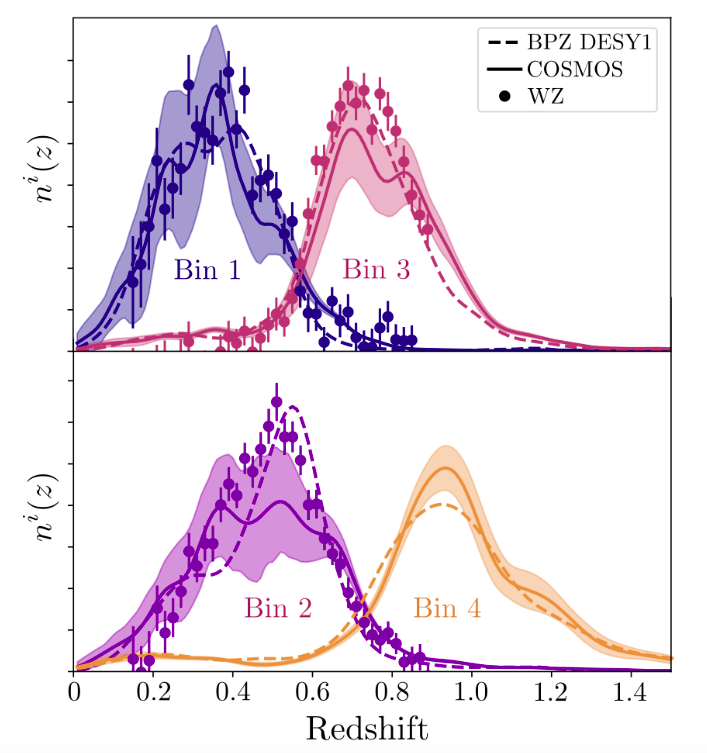
\includegraphics[width=\linewidth]{dndz-fig4.png}
                \newline
                {\tiny Hoyle et al. 2018}
        \end{column}

    \end{columns}

}

\frame
{

    \frametitle{DES Year 1 Cosmology Results}

    %\setbeamerfont*{itemize/enumerate body}{size=\large}

    \begin{columns}
        \begin{column}{0.5\textwidth}
            \begin{itemize}

                \item These combined shear and galaxy clustering signals
                    are then fit simultaneously to constrain cosmological
                    parameters.

                \item The most accurate and precise cosmological
                    constraints to date using weak lensing.


            \end{itemize}

        \end{column}
        \begin{column}{0.5\textwidth}
            \centering
                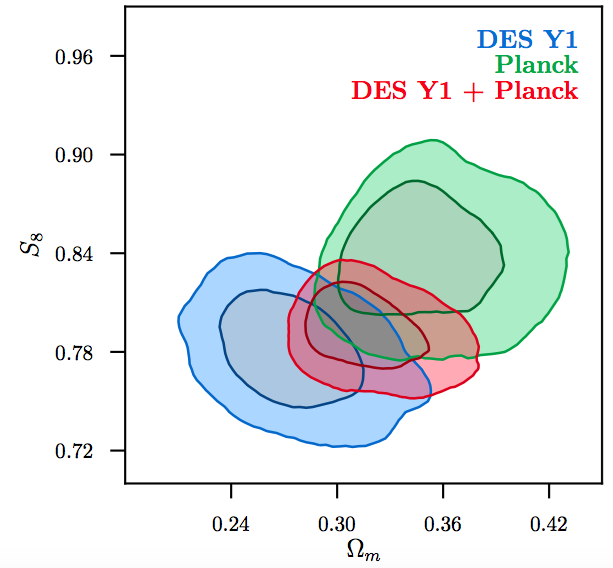
\includegraphics[width=\linewidth]{3x2-fig10.png}
                \newline
                {\tiny DES Collaboration 2018}
        \end{column}

    \end{columns}

}


\frame
{

    \frametitle{DES Year 1 Cosmology Results}

    %\setbeamerfont*{itemize/enumerate body}{size=\large}

    \begin{columns}
        \begin{column}{0.5\textwidth}
            \begin{itemize}

                \item Measurements agree with those from the
                    Planck Cosmic Microwave Background measurements
                    as well as Baryonic Acoustic Oscillation
                    and Supernova measurements.

                \item The combination  of all these probes gives
                    our best constraints to date of the properties
                    Dark Energy

            \end{itemize}

        \end{column}
        \begin{column}{0.5\textwidth}
            \centering
                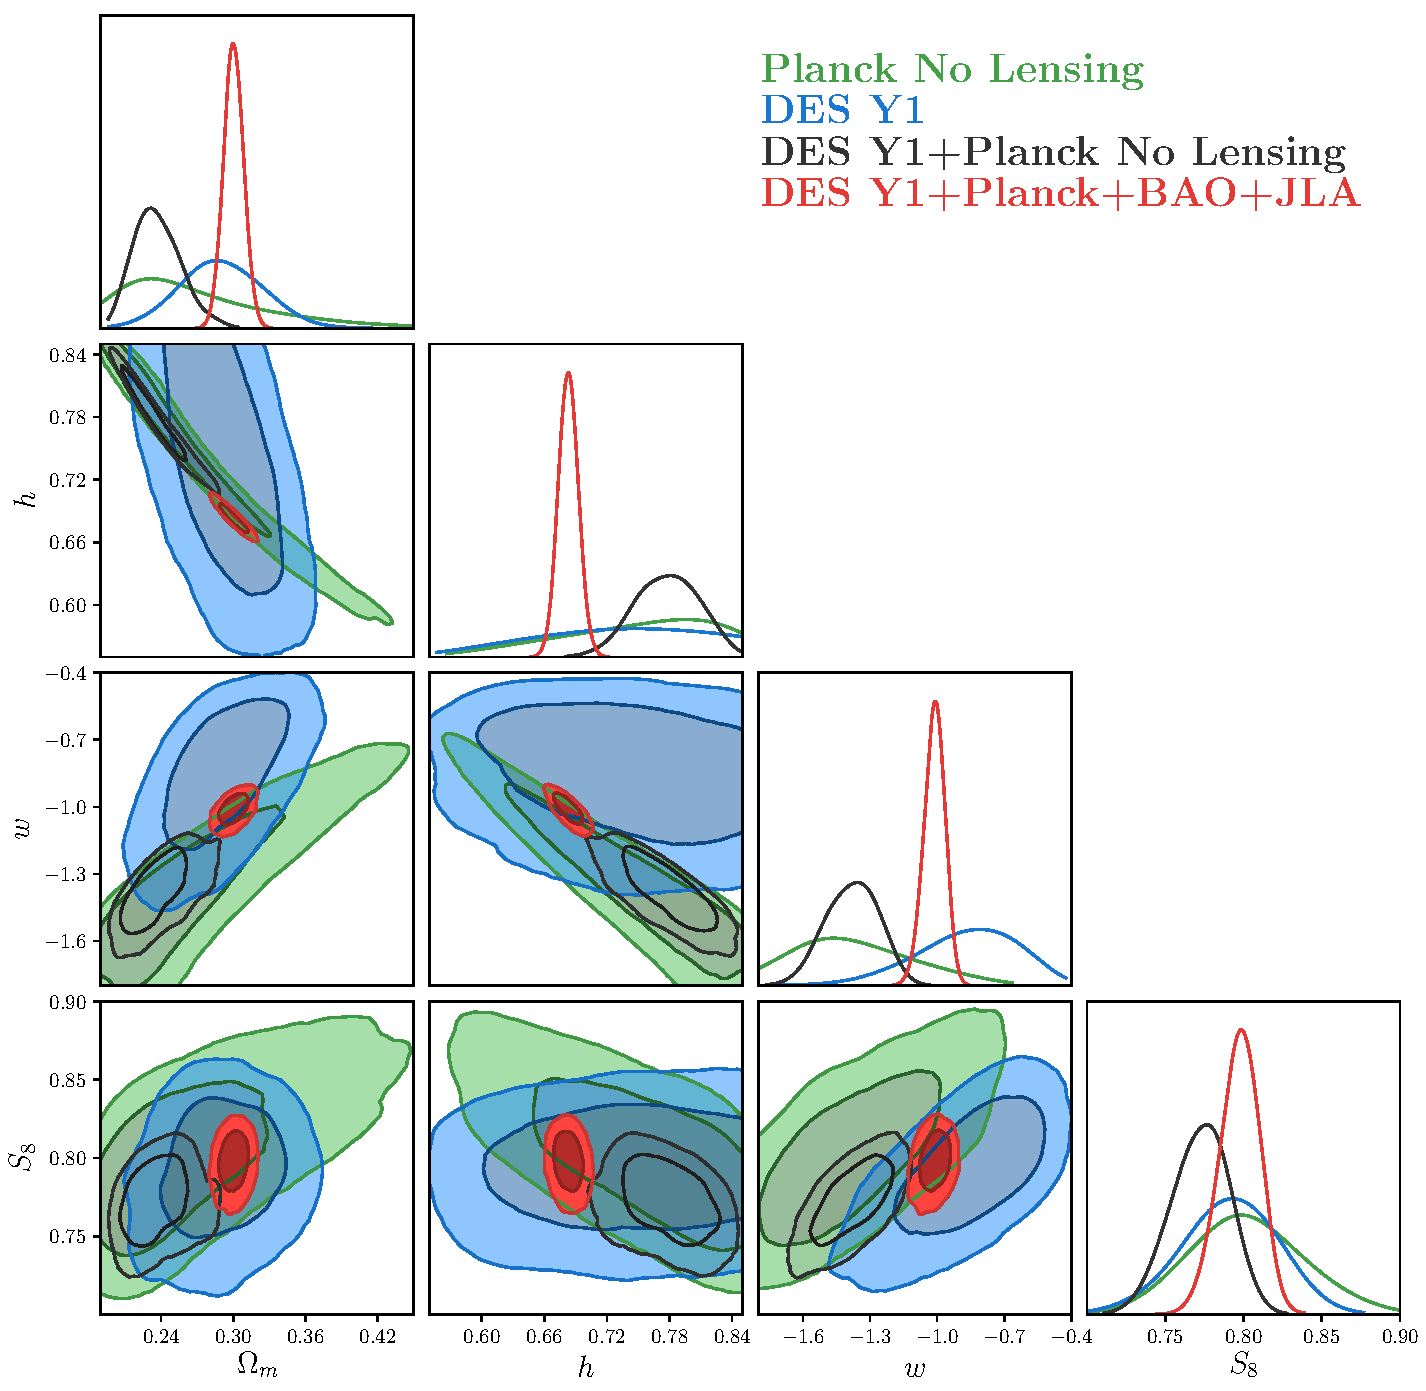
\includegraphics[width=\linewidth]{dpnl_w_4.pdf}
                \newline
                {\tiny DES Collaboration 2018}
        \end{column}

    \end{columns}

}

\frame
{

    \frametitle{DES Year 3 Analysis}

    %\setbeamerfont*{itemize/enumerate body}{size=\large}

    \begin{columns}
        \begin{column}{0.5\textwidth}
            \begin{itemize}

                \item DES Year 3 analysis is under way

                \item Large increase in area over Year 1, with
                    comparable depth.

                \item The MOF deblender processing was completed
                    last year.

                \item Finalizing shear catalog now.


            \end{itemize}

        \end{column}
        \begin{column}{0.5\textwidth}
            \centering
                \includegraphics[width=\linewidth]{{y3a2_gold_1.0_auto_v1.1_depth_Y}.png}
                \newline
                {\tiny Year 3 Galaxy Depth}
        \end{column}

    \end{columns}

}

\frame
{

    \frametitle{DES Year 3 and Year 5}

    %\setbeamerfont*{itemize/enumerate body}{size=\large}

    \begin{itemize}

        \item Year 3 is three times the area of year 1 at the same depth:  expect
            $\sqrt 3$ times improvement in the precision of the lensing measurements,
            with corresponding improvement in cosmological parameters.

        \item Year 5 covers roughly the same area as year 3 but at greater depth.
            With the greater depth the number density of detected galaxies increases significantly.
            We expect a roughly $\sqrt 2$ improvement beyond year 3.

        \item Codes now incorporated into standard data management system. For
            year 5 these measurements will be made as part of standard
            processing.

    \end{itemize}

}


\frame
{

    \frametitle{Summary}

    %\setbeamerfont*{itemize/enumerate body}{size=\large}

    \begin{columns}
        \begin{column}{0.5\textwidth}
            \begin{itemize}

                \item DES Year 1 results provide the best
                    cosmological constraints to date using
                    weak gravitational lensing

                \item BNL has made fundamental contributions to this work by
                    providing the shear and basic object photometry used in
                    all measurements.

                \item DES Year 3 analysis is proceeding, expect exciting
                    new results soon!

            \end{itemize}

        \end{column}
        \begin{column}{0.5\textwidth}
            \centering
                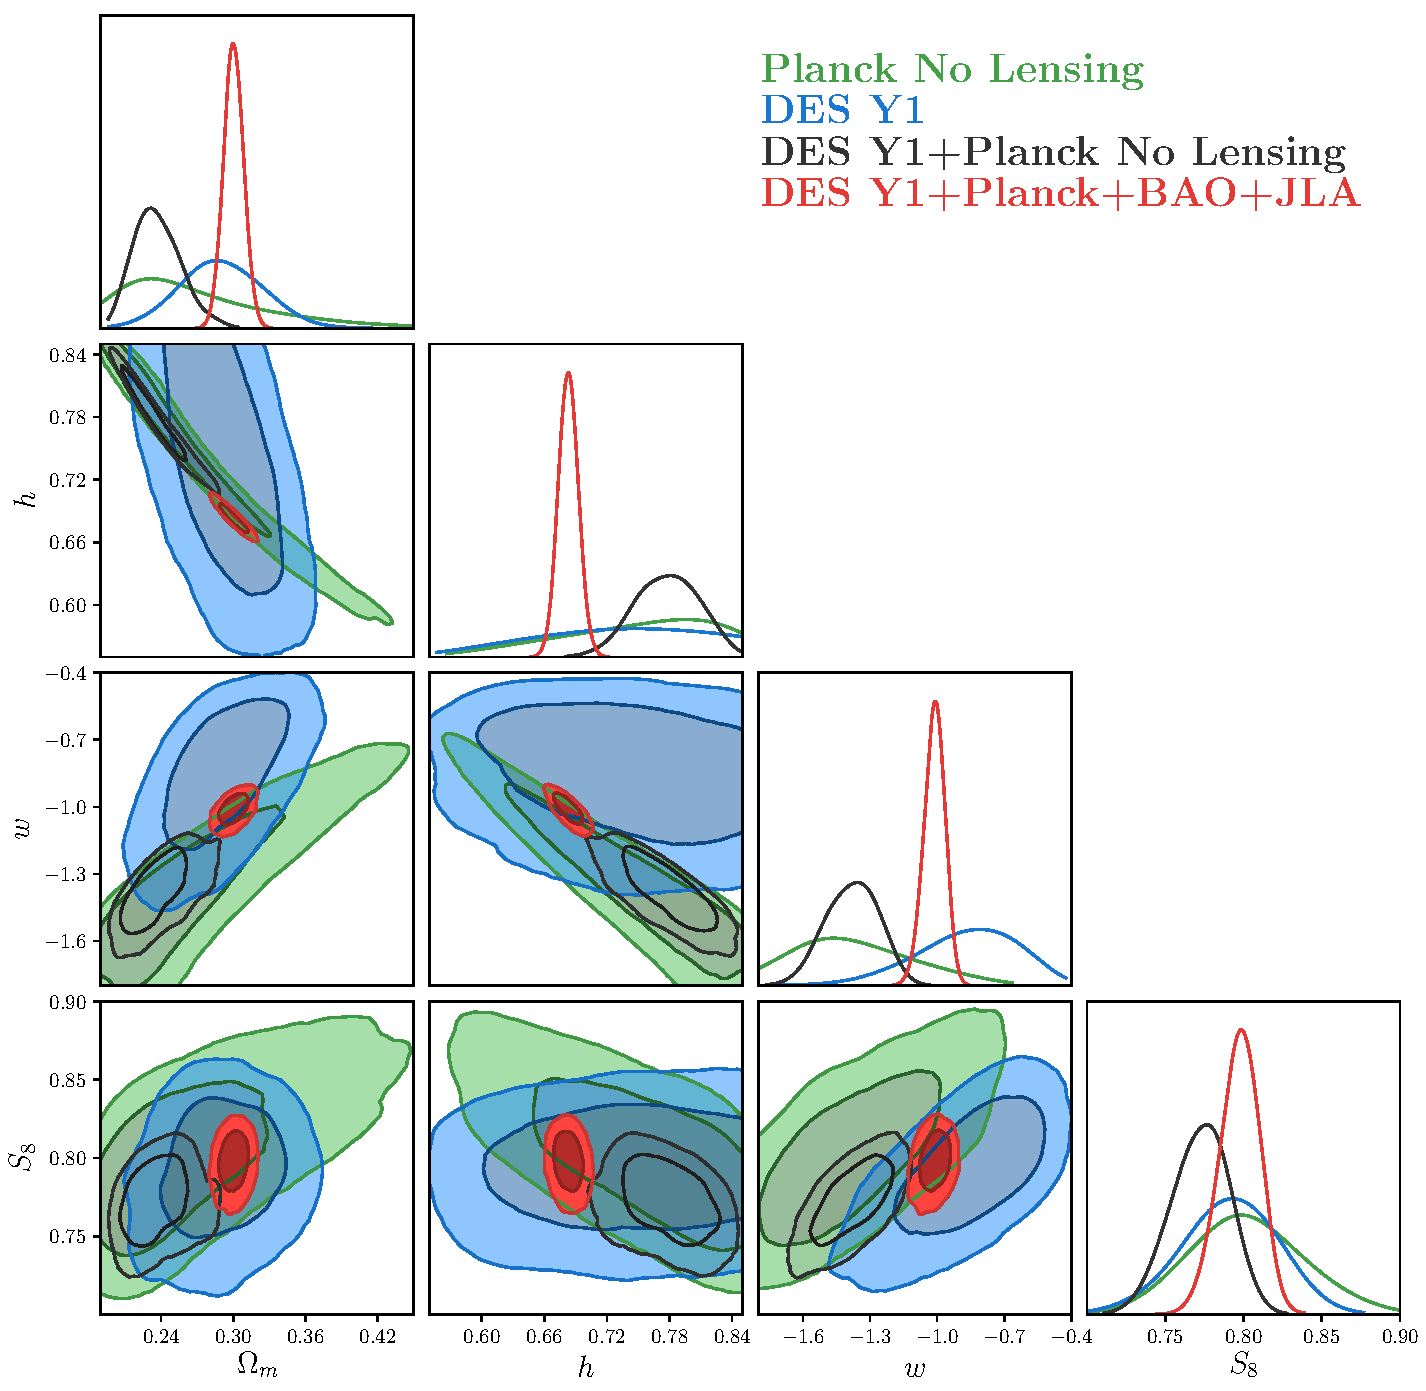
\includegraphics[width=\linewidth]{dpnl_w_4.pdf}
                \newline
                {\tiny DES Collaboration 2018}
        \end{column}

    \end{columns}

}








\end{document}
